\documentclass[notes=show,handout]{beamer}\usepackage[]{graphicx}\usepackage[]{color}
% maxwidth is the original width if it is less than linewidth
% otherwise use linewidth (to make sure the graphics do not exceed the margin)
\makeatletter
\def\maxwidth{ %
  \ifdim\Gin@nat@width>\linewidth
    \linewidth
  \else
    \Gin@nat@width
  \fi
}
\makeatother

\definecolor{fgcolor}{rgb}{0.345, 0.345, 0.345}
\newcommand{\hlnum}[1]{\textcolor[rgb]{0.686,0.059,0.569}{#1}}%
\newcommand{\hlstr}[1]{\textcolor[rgb]{0.192,0.494,0.8}{#1}}%
\newcommand{\hlcom}[1]{\textcolor[rgb]{0.678,0.584,0.686}{\textit{#1}}}%
\newcommand{\hlopt}[1]{\textcolor[rgb]{0,0,0}{#1}}%
\newcommand{\hlstd}[1]{\textcolor[rgb]{0.345,0.345,0.345}{#1}}%
\newcommand{\hlkwa}[1]{\textcolor[rgb]{0.161,0.373,0.58}{\textbf{#1}}}%
\newcommand{\hlkwb}[1]{\textcolor[rgb]{0.69,0.353,0.396}{#1}}%
\newcommand{\hlkwc}[1]{\textcolor[rgb]{0.333,0.667,0.333}{#1}}%
\newcommand{\hlkwd}[1]{\textcolor[rgb]{0.737,0.353,0.396}{\textbf{#1}}}%
\let\hlipl\hlkwb

\usepackage{framed}
\makeatletter
\newenvironment{kframe}{%
 \def\at@end@of@kframe{}%
 \ifinner\ifhmode%
  \def\at@end@of@kframe{\end{minipage}}%
  \begin{minipage}{\columnwidth}%
 \fi\fi%
 \def\FrameCommand##1{\hskip\@totalleftmargin \hskip-\fboxsep
 \colorbox{shadecolor}{##1}\hskip-\fboxsep
     % There is no \\@totalrightmargin, so:
     \hskip-\linewidth \hskip-\@totalleftmargin \hskip\columnwidth}%
 \MakeFramed {\advance\hsize-\width
   \@totalleftmargin\z@ \linewidth\hsize
   \@setminipage}}%
 {\par\unskip\endMakeFramed%
 \at@end@of@kframe}
\makeatother

\definecolor{shadecolor}{rgb}{.97, .97, .97}
\definecolor{messagecolor}{rgb}{0, 0, 0}
\definecolor{warningcolor}{rgb}{1, 0, 1}
\definecolor{errorcolor}{rgb}{1, 0, 0}
\newenvironment{knitrout}{}{} % an empty environment to be redefined in TeX

\usepackage{alltt}
\usepackage{amsmath}
\usepackage{graphicx}
\usepackage{mathpazo}
\usepackage{hyperref}
\usepackage{multimedia}
\usepackage{epstopdf}
\setcounter{MaxMatrixCols}{10}
\usetheme{Madrid}
\usepackage{multicol}
\usepackage{multimedia}
\usepackage{epstopdf}
\usepackage{tikz}
\usetikzlibrary{shapes,backgrounds}


\newtheorem{conj}{Conjecture}[section]
\newtheorem{aim}{Aim}[section]

\newtheorem{remark}{Remark}[section]
\newtheorem{proposition}{Proposition}[section]
\newtheorem{interpretation}{Interpretation}[section]
\newtheorem{goal}{Goal}[section]
\newtheorem{exercise}{Exercise}[section]

\newcommand{\mbf}[1]{\mathbf{#1}}
\newcommand{\beq}{\begin{equation}}
\newcommand{\eeq}{\end{equation}}
\newcommand{\bea}{\begin{eqnarray}}
\newcommand{\eea}{\end{eqnarray}}
\newcommand{\ba}{\begin{array}}
\newcommand{\ea}{\end{array}}
\newcommand{\bi}{\begin{itemize}}
\newcommand{\ei}{\end{itemize}}
\newcommand{\ben}{\begin{enumerate}}
\newcommand{\een}{\end{enumerate}}
\newcommand{\nn}{\nonumber}
\newcommand{\fn}[1]{\footnote{#1}}
\renewcommand{\r}{\right}
\renewcommand{\l}{\left}
\long\def\symbolfootnote[#1]#2{\begingroup\def\thefootnote{\fnsymbol{footnote}}\footnote[#1]{#2}\endgroup}


%%%%%%%%%%%%%%%%%%%%%%%%%%%%%%%%%%%%%%%%%%%%%%%%%%%%%%%%%%%%%%%%%%%%%%%%%%%%%%%
% GSEM COLORS
%%%%%%%%%%%%%%%%%%%%%%%%%%%%%%%%%%%%%%%%%%%%%%%%%%%%%%%%%%%%%%%%%%%%%%%%%%%%%%%
\definecolor{darkGSEM}{RGB}{70,95,127}
\definecolor{darkGSEM2}{RGB}{40,80,150}
\definecolor{GSEM}{RGB}{96,121,153} % GSEM 10% lighter

%%% Global colors
\setbeamercolor*{palette primary}{use=structure,fg=white,bg=darkGSEM}
\setbeamercolor*{palette quaternary}{use=structure,fg=white,bg=darkGSEM!90}
\setbeamercolor{frametitle}{fg=white,bg=GSEM!80}

%%% TOC colors
\setbeamercolor{section in toc}{fg=darkGSEM}

%%% itemize colors
\setbeamertemplate{itemize items}[circle]
\setbeamercolor{itemize item}{fg=darkGSEM2}
\setbeamercolor{itemize subitem}{fg=darkGSEM2}
\setbeamercolor{itemize subsubitem}{fg=darkGSEM2}


%%% enumerate colors
\setbeamercolor{item projected}{fg=white,bg=GSEM}
\setbeamertemplate{enumerate item}{\insertenumlabel.}
\setbeamercolor{enumerate item}{fg=darkGSEM2}
\setbeamercolor{enumerate subitem}{fg=darkGSEM2}
\setbeamercolor{enumerate subsubitem}{fg=darkGSEM2}


\AtBeginSection[]
{
  \begin{frame}
    \frametitle{Outline}
    \tableofcontents[currentsection]
  \end{frame}
}

%%%%%%%%%%%%%%%%%%%%%%%%%%%%%%%%%%%%%%%%%%%%%%%%%%%%%%%%%%%%%%%%%%%%%%%%%%%%%%%%
\IfFileExists{upquote.sty}{\usepackage{upquote}}{}
\begin{document}

\title[S110015]{Probability 1}
\subtitle{Lecture 03 : Probability Axioms}
\author[Flores-Agreda, La Vecchia]{Dr. Daniel Flores-Agreda, \\[0.5em] \tiny{(based on the notes of Prof. Davide La Vecchia)}}
\date{Spring Semester 2021}

\begin{frame}
  \titlepage
\end{frame}

\begin{frame}{Objective}
  \begin{itemize}
  \item Provide the Axioms upon which the Probability Theory is built.
  \item Explore some rules that result from the Axioms
  \item Illustrate how these rules can be used to compute probabilities ``in real life''
  \item Introduce the concepts of Independence and Conditional Probability
  \item Present two important Theorems and illustrate their consequences.
  \end{itemize}
\end{frame}

\begin{frame}{Outline}
\tableofcontents
\end{frame}

%%%%%%%%%%%%%%%%%%%%%%%%%%%%%%%%%%%%%%%%%%%%%%%%%%%%%%%%%%%%%%%%%%%%%%%%%%%%%%%%
\section{An Axiomatic Definition of Probability}
%%%%%%%%%%%%%%%%%%%%%%%%%%%%%%%%%%%%%%%%%%%%%%%%%%%%%%%%%%%%%%%%%%%%%%%%%%%%%%%%

\begin{frame}{\secname}
  %Let $\mathcal{B}$ be the $\sigma$-algebra of subsets of a set $S$ representing the sample space. \\
  %\vspace{0.1cm}
  \begin{definition}
  We define probability a set function with values in $[0,1]$, which
  satisfies the following axioms:
  \begin{itemize}
  \item[ (i)] $P(A) \geq 0$, for every event $A$
  \item[ (ii)] $P(S)=1$
  \item[ (iii)] If $A_1,A_2,...$ is a sequence of mutually exclusive events (namely \color{red}$A_i \cap A_j =\varnothing$, for $i \neq j$, and $i,j=1,2,...$\color{black}),
  and such that
  $A = \bigcup_{i=1}^{\infty} A_i$, then
  \bea
  \label{Eq: additivity}
  P(A) &=& P\left(  \bigcup_{i=1}^\infty A_i \right) = \sum_{i=1}^{\infty} P(A_i).
  \eea
  \end{itemize}
  \end{definition}
\end{frame}

%%%%%%%%%%%%%%%%%%%%%%%%%%%%%%%%%%%%%%%%%%%%%%%%%%%%%%%%%%%%%%%%%%%%%%%%%%%%%%%%
\section{Implications: Properties of $P(\cdot)$}
%%%%%%%%%%%%%%%%%%%%%%%%%%%%%%%%%%%%%%%%%%%%%%%%%%%%%%%%%%%%%%%%%%%%%%%%%%%%%%%%

\begin{frame}{\secname}
  We can use the three axioms to build more sophisticated statements, e.g.
  \bigskip
  \begin{itemize}
  \item The Probability of the Empty Set
  \item The Addition Law of Probability
  \item The Complement Rule
  \item The Monotonicity Rule
  \item The Probability of the Union
  \item Boole's Inequality
  \end{itemize}
\end{frame}

\begin{frame}{\secname}
  \begin{theorem}[Probability of the Empty Set]
  $$P(\varnothing)=0$$
  \end{theorem}
  \pause
  \begin{proof}
  \begin{footnotesize}
  Take $A_1=A_2=A_3=....=\varnothing$. Then by (\ref{Eq: additivity}) in Axiom (ii) we have
  $$
  P(\varnothing)= P\left(  \bigcup_{i=1}^{\infty} A_i \right)
  = \sum_{i=1}^{\infty} P(A_i)
  =\sum_{i=1}^{\infty} P(\varnothing)
  $$
  which is true only if it is an infinite sum of zeros. Thus
  $$
  P(\varnothing) =  0.
  $$
  \end{footnotesize}
  \end{proof}
\end{frame}

\begin{frame}{\secname}
  \begin{theorem}[The Addition Law of Probability]
  If $A_1, A_2,...$ are mutually exclusive events, then
  \begin{equation}
  P\left(  \bigcup_{i=1}^{n} A_i \right) = \sum_{i=1}^{n} P(A_i).  \label{Eq: ProbUnionDisj}
  \end{equation}
  \end{theorem} %\vspace{0.1cm}

  \pause

  \begin{footnotesize}
  \begin{proof}
  Let $A_{n+1}=A_{n+2}=....=\varnothing$, then
  $
  \bigcup_{i=1}^{n} A_i = \bigcup_{i=1}^{\infty} A_i,
  $
  and, from (\ref{Eq: additivity}) (see Axiom (iii)) it follows
  \bea
  P\left(  \bigcup_{i=1}^{n} A_i \right) &=& P\left(  \bigcup_{i=1}^{\infty} A_i \right)
  = \sum_{i=1}^{\infty} P(A_i) = \sum_{i=1}^{n} P(A_i) + \underbrace{\sum_{i=n+1}^{\infty} P(A_i)}_{\equiv 0}. \nn
  \eea
  \end{proof}
  \end{footnotesize}
\end{frame}

\begin{frame}{\secname}
  \begin{theorem}[The Complement Rule]
  If $A$ is an event, then
  $
  P(  A^c ) = 1- P(A).
  $
  \end{theorem} \vspace{0.1cm}


  \begin{footnotesize}
  \begin{proof}
  Let $A \cup A^c =S$ and $A \cap A^c = \varnothing$, so
  and
  $$
  P( S ) = P\left(A \cup A^c \right) =P(A) + P\left(A^c \right). \nn
  $$
  By Axiom (i) Axiom (ii) we have $P(S)=1$, so the desired result follows from:
  $$
  1 = P(A) + P\left(A^c \right).
  $$
  \end{proof}
  \end{footnotesize}
\end{frame}


%\begin{frame}
%\frametitle{Properties of $P(\cdot)$ (cont'd)}
%Assume we have two events $A \in \mathcal{B}$ and $B \in \mathcal{B}$, such that $B \subset A$. Graphically,
%we are in the following setting:
%\vspace{0.2cm} \hspace{0.3cm}
%
%\begin{tikzpicture}
%    \begin{scope}[shift={(1cm,-3cm)}, fill opacity=0.55]
%        \draw[fill=red, draw = black] (0,0) circle (3);
%        \draw[fill=green, draw = black] (-0.5,0) circle (2);
%    \node at (0,2.2) (A) {\large\textbf{A}};
%    \node at (-0.15,-0.25) (B) {\large\textbf{B}};
%    \end{scope}
%
%\end{tikzpicture}
%\end{frame}
%

\begin{frame}{\secname}
  \begin{theorem}[The Monotonicity Rule]
  For any two events $A$ and $B$, such that $B \subset A$, we have
  $$
  P(A) \geq P(B).
  $$
  \end{theorem} \vspace{0.1cm}
  \begin{footnotesize}
  \begin{proof}
  Let us write
  $$A = B \cup (B^c \cap A) $$
  and notice that $B \cap (B^c \cap A) = \phi$, so that
  \bea
  P(A) &=& P\left\{ B \cup (B^c \cap A)   \right\} \nn \\
  &=& P(B) + P(B^c \cap A) \nn
  \eea
  which implies (since $P(B^c \cap A) \geq 0$) that
  $$
  P(A) \geq   P(B).
  $$

  \end{proof}
  \end{footnotesize}
\end{frame}

\begin{frame}{\secname}
  \def\firstcircle{(3,1) circle (2.95cm)}
  \def\secondcircle{(1:3cm) circle (1.65cm)}

  \colorlet{circle edge}{blue!50}
  \colorlet{circle area}{blue!20}
  \tikzset{filled/.style={fill=circle area, draw=circle edge, thick},
      outline/.style={draw=circle edge, thick}}
  \hspace{3cm} \vspace{2cm}
  \begin{tikzpicture}
      \draw[even odd rule] \firstcircle node at (1.95,1.9) {$A$}
                                   \secondcircle node at (2.5,0.5) {$B$};
      \node[anchor=south] at (current bounding box.north) at (6.5,2.2) {$B \subset A$};
  \end{tikzpicture}
  %where $A \in \mathcal{B}$ and $B \in \mathcal{B}$
  \begin{center}
  In some sense, Probability works like areas.
  \end{center}
\end{frame}


\begin{frame}{\secname}
  \begin{theorem}[Probability of the Union of Two Events]
  For any two events $A$ and $B$ then
  $$
  P(A \cup B) = P(A) + P(B) - P(A \cap B).
  $$
  \end{theorem}
  \vspace{0.1cm}
  \begin{footnotesize}
  \begin{proof}
  Consider that $A\cup B = A \cup (A^c \cap B)$, and $A\cap(A^c \cap B) = \phi$. Now remember\footnote{See Lecture 1 for the meaning of set difference.} that $A^c \cap B = B -(A \cap B)$, so,
  \bea
  P(A\cup B) &=& P(A) + P(A^c \cap B) \nn \\
  &=& P(A) + P(B) - P(A\cap B). \nn
  \eea

  \end{proof}
  \end{footnotesize}
\end{frame}


\begin{frame}{\secname}
  \begin{theorem} [Boole's inequality]
  For the events $A_1,A_2,... A_n$,
  $$
  P(A_1 \cup A_2 \cup....\cup A_n) \leq \sum_{i=1}^{n}P(A_i).
  $$
  \end{theorem}
  \vspace{0.1cm}
  %\begin{footnotesize}
  %\begin{proof}
  For instance, let us consider $n=2$. Then we have:
  $$
  P(A_1 \cup A_2 ) = P(A_1) + P(A_2) - P(A_1 \cap A_2) \leq P(A_1) + P(A_2)
  $$
  since $P(A_1 \cap A_2) \geq 0$ by definition.
  %\end{proof}
  %\end{footnotesize}
  \begin{remark}
  It is worth notice that if $A_j \cap A_i = \varnothing$, for every $i$ and $j$, with $i\neq j$, then
  $
  P(A_1 \cup A_2 \cup....\cup A_n) = \sum_{i=1}^{n}P(A_i),
  $
  as stated in (\ref{Eq: ProbUnionDisj}).
  \end{remark}
\end{frame}

%%%%%%%%%%%%%%%%%%%%%%%%%%%%%%%%%%%%%%%%%%%%%%%%%%%%%%%%%%%%%%%%%%%%%%%%%%%%%%%%
\section{Examples and Illustrations}
%%%%%%%%%%%%%%%%%%%%%%%%%%%%%%%%%%%%%%%%%%%%%%%%%%%%%%%%%%%%%%%%%%%%%%%%%%%%%%%%

\begin{frame}{\secname}
  \begin{example}[Flipping a coin twice]
    \begin{footnotesize}
    \textbf{If we flip a balanced coin twice, {what is the probability of getting at least one head?}}

    \begin{itemize}
    \item The sample space is: $S = \{HH, HT, TH, TT\}$
    \item Balanced coin: outcomes are equally likely and $p_{HH} = p_{HT} = p_{TH} = p_{TT} = p = 1/4$
    \item Let $A$ denote the event \textbf{obtaining at least one Head}, i.e. $H = \{HH, HT, TH\}$
    \end{itemize}
    \begin{align*}
    Pr(A) &= Pr(\{HH \cup HT \cup TH\}) \\
          &= Pr(\{HH\}) +   Pr(\{HT\}) + Pr(\{TH\})\\
          &= \frac{1}{4} +\frac{1}{4}+\frac{1}{4} = \frac{3}{4}
    \end{align*}
    \end{footnotesize}
  \end{example}
\end{frame}

\begin{frame}{\secname}
  \begin{example}[Detecting Shoppers]
      \begin{footnotesize}
      \textit{Shopper TRK is an electronic device that counts the number of shoppers entering a shopping centre.}

      \textit{Two shoppers enter the shopping centre together, one walking in front of the other:}

      \begin{enumerate}
      \item \textit{There is a 0.98 probability that the first shopper is detected}
      \item \textit{There is a 0.94 probability that the second shopper is detected}.
      \item \textit{There is a 0.93 probability that both shoppers are detected}.
      \end{enumerate}
      \textbf{What is the probability that the device will detect at least one of the two shoppers entering?}
    \end{footnotesize}
  \end{example}
\end{frame}

\begin{frame}{\secname}
  \begin{example}[Detecting Shoppers, continued]
    \begin{footnotesize}
      Define the \textbf{events}:

      \begin{itemize}
      \item $D$ (shopper is detected) and
      \item $U$ (shopper is undetected).
      \end{itemize}

      Then, the Sample Space is $S=\{ DD, DU, UD, UU\}$

      Define the \textbf{probabilities}:
      \begin{itemize}
      \item $Pr(DD \cup DU) = 0.98$
      \item $Pr(DD \cup UD) = 0.94$
      \item $Pr(DD) = 0.93$
      \end{itemize}
    \end{footnotesize}
  \end{example}
\end{frame}

\begin{frame}{\secname}
  \begin{example}[Detecting Shoppers, continued]

  \begin{footnotesize}
  \begin{align*}
  Pr(DD \cup UD \cup DU) &= Pr(\{DD \cup UD\} \cup \{DD \cup DU\})\\
  &= Pr(\{DD \cup UD\}) + Pr(\{DD \cup DU\})\\
  &- Pr(\{DD \cup UD\} \cap \{DD \cup DU\})
  \end{align*}

  The only missing probability is : $P\{DD \cup UD\} \cap \{DD \cup DU\} = ?$

  To compute it, let's use the fact that \textbf{the union is distributive with respect to the intersection} (see Ch 2):

  $$(DD \cup UD) \cap (DD \cup DU) = DD \cup (UD \cap DU) =DD \cup \varnothing = DD$$
  \end{footnotesize}
  \end{example}
\end{frame}

\begin{frame}{\secname}
  \begin{example}[Detecting Shoppers, continued]
  \begin{footnotesize}
  Graphically:
  \begin{figure}[h!]
  \centering
  \includegraphics[scale = 0.1]{../../book/img/03_axioms/Example2_3_v2.png}
  \end{figure}

  So, the desired probability is:
  \begin{align*}
    Pr(DD \cup UD \cup DU) &= Pr(\{DD \cup UD\}) + Pr(\{DD \cup DU\}) - Pr(DD) \\
    &= 0.98 + 0.94-0.93 \\
    &= 0.99
  \end{align*}
  \end{footnotesize}
  \end{example}
\end{frame}


\begin{frame}{\secname}
  \begin{example}[De Morgan's law]
  \begin{small}
  Given  $P(A\cup B)=0.7$ and $P(A\cup {B}^c) = 0.9$, find $P(A)$.


  \vspace{0.2cm}


  By De Morgan's law,
  $$P(A^c \cap B^c) = P((A\cup B )^c) = 1 - P(A\cup B) = 1 - 0.7 = 0.3$$
  and similarly
  $$P(A^c \cap B) = 1 - P(A \cup B^c) = 1- 0.9 = 0.1.$$

  Thus,
  $$P(A^c)=P(A^c \cap B^c )+P(A^c \cap B)= 0.3+ 0.1= 0.4,$$

  so
  $$P(A)=1 - 0.4= 0.6.$$
  \end{small}
   \end{example}
\end{frame}


\begin{frame}{\secname}

  \begin{example}[Probability, union, and complement]
  \begin{small}
  \textit{John is taking two books along on his holiday vacation. With probability 0.5, he will like the first book; with probability 0.4, he will like the
  second book; and with probability 0.3, he will like both books. What is the probability that he likes neither book?}

  \vspace{0.2cm}

  \begin{footnotesize}
  Let $A_i$ be the event that John likes book $i$, for $i=1,2$. Then the probability that he likes at least one book is:
  \bea
  P(\bigcup_{i=1}^2 A_i) &=& P(A_1 \cup A_2) = P(A_1) + P(A_2) - P(A_1\cap A_2) \nn \\
  &=& 0.5 + 0.4 -0.3 =0.6. \nn
  \eea
  Because the event the John likes neither books is the complement of the event that he likes at leas one of them (namely $A_1 \cup A_2$), we have
  $$
  P(A^{c}_1 \cap A^{c}_2 ) = P((A_1 \cup A_2)^c) = 1- P (A_1 \cup A_2) = 0.4.
  $$
  \end{footnotesize}
  \end{small}
  \end{example}
\end{frame}

% \begin{frame}{\secname}
%   \begin{example}[Temperatures]
%   \begin{small}
%   \textit{Let $A$ denote the event that the midtown temperature in Los Angeles (LA) is 70 F, $B$ the event that the midtown temperature in New York (NY) is 70 F, and $C$ the event that the maximum of midtown temperatures in NY and LA is 70 F.}
%   \textit{If $P(A)=0.3, \ P(B)=0.4, \text{and} P(C)=0.2$, find the probability that the minimum of the two midtown temperatures is 70 F}.
%   \end{small}
%   \end{example}
% \end{frame}
%
% \begin{frame}{\secname}
%   \begin{example}[Temperatures, cont'd]
%   \begin{small}
%
%   \vspace{0.2cm}
%   Let $D$ denote the event that the minimum temperature is 70 F. Then
%   \bea
%   P(A\cup B) &=& P(A) + P(B) - P(AB) = 0.7 -P(AB) \nn \\
%   P(C\cup D) &=& P(C) + P(D) - P(CD) = 0.2 -P(D) - P(DC). \nn
%   \eea
%   Since $$A\cup B = C \cup D \quad \text{and} \quad A\cap B = C\cap D,$$
%   subtracting one of the preceding equations from the other we get
%   \begin{eqnarray*}
%   P(A\cup B)-P(C\cup D)  & = &  0.7 -P(AB) - [0.2 -P(D) - P(D\cap C)] \\
%   &  = & 0.5 -P(D) = 0 , \\
%   \end{eqnarray*}
%   thus $ P(D) =0.5.$
%   \end{small}
%   \end{example}
% \end{frame}

%%%%%%%%%%%%%%%%%%%%%%%%%%%%%%%%%%%%%%%%%%%%%%%%%%%%%%%%%%%%%%%%%%%%%%%%%%%%%%%%
\section{Conditional Probability}
%%%%%%%%%%%%%%%%%%%%%%%%%%%%%%%%%%%%%%%%%%%%%%%%%%%%%%%%%%%%%%%%%%%%%%%%%%%%%%%%

\begin{frame}{\secname}
  \begin{figure}[h!]
  \centering
  \includegraphics[scale=2]{../../book/img/fun/probconditionnelle2.png}
  \end{figure}
\end{frame}


\begin{frame}{\secname}
Sometimes, probability depends on the information available.
  \begin{example}
  Suppose you have two dice and throw them; the possible outcomes are:
  \begin{figure}[h!]
  \centering
  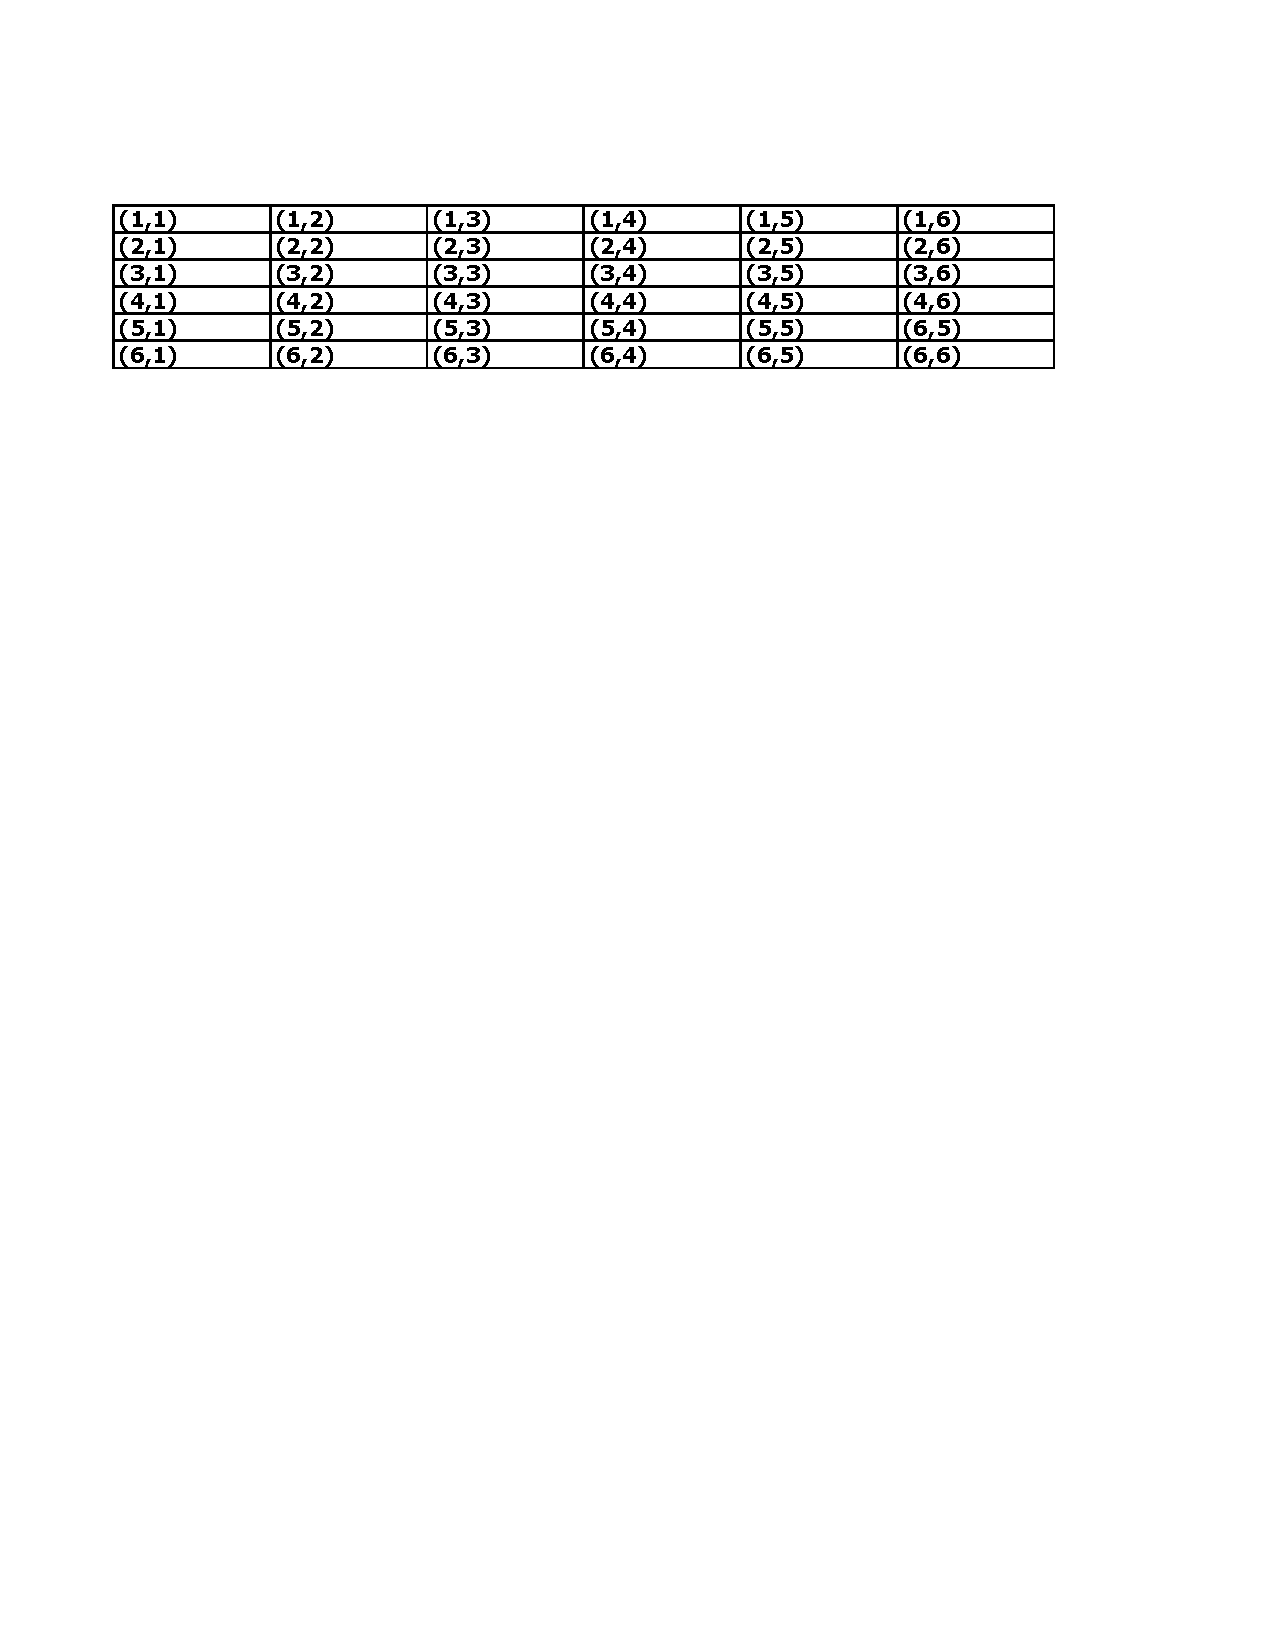
\includegraphics[scale=0.7]{img/c1.pdf}
  \end{figure}
  \end{example}
\end{frame}


\begin{frame}{\secname}

  \begin{example}[cont'd]
  Consider the event $A$ = getting $5$, or equivalently $A=\{ 5\}$.

  What is $P(A)$, namely, the probability of getting $5$?

  \begin{figure}[h!]
  \centering
  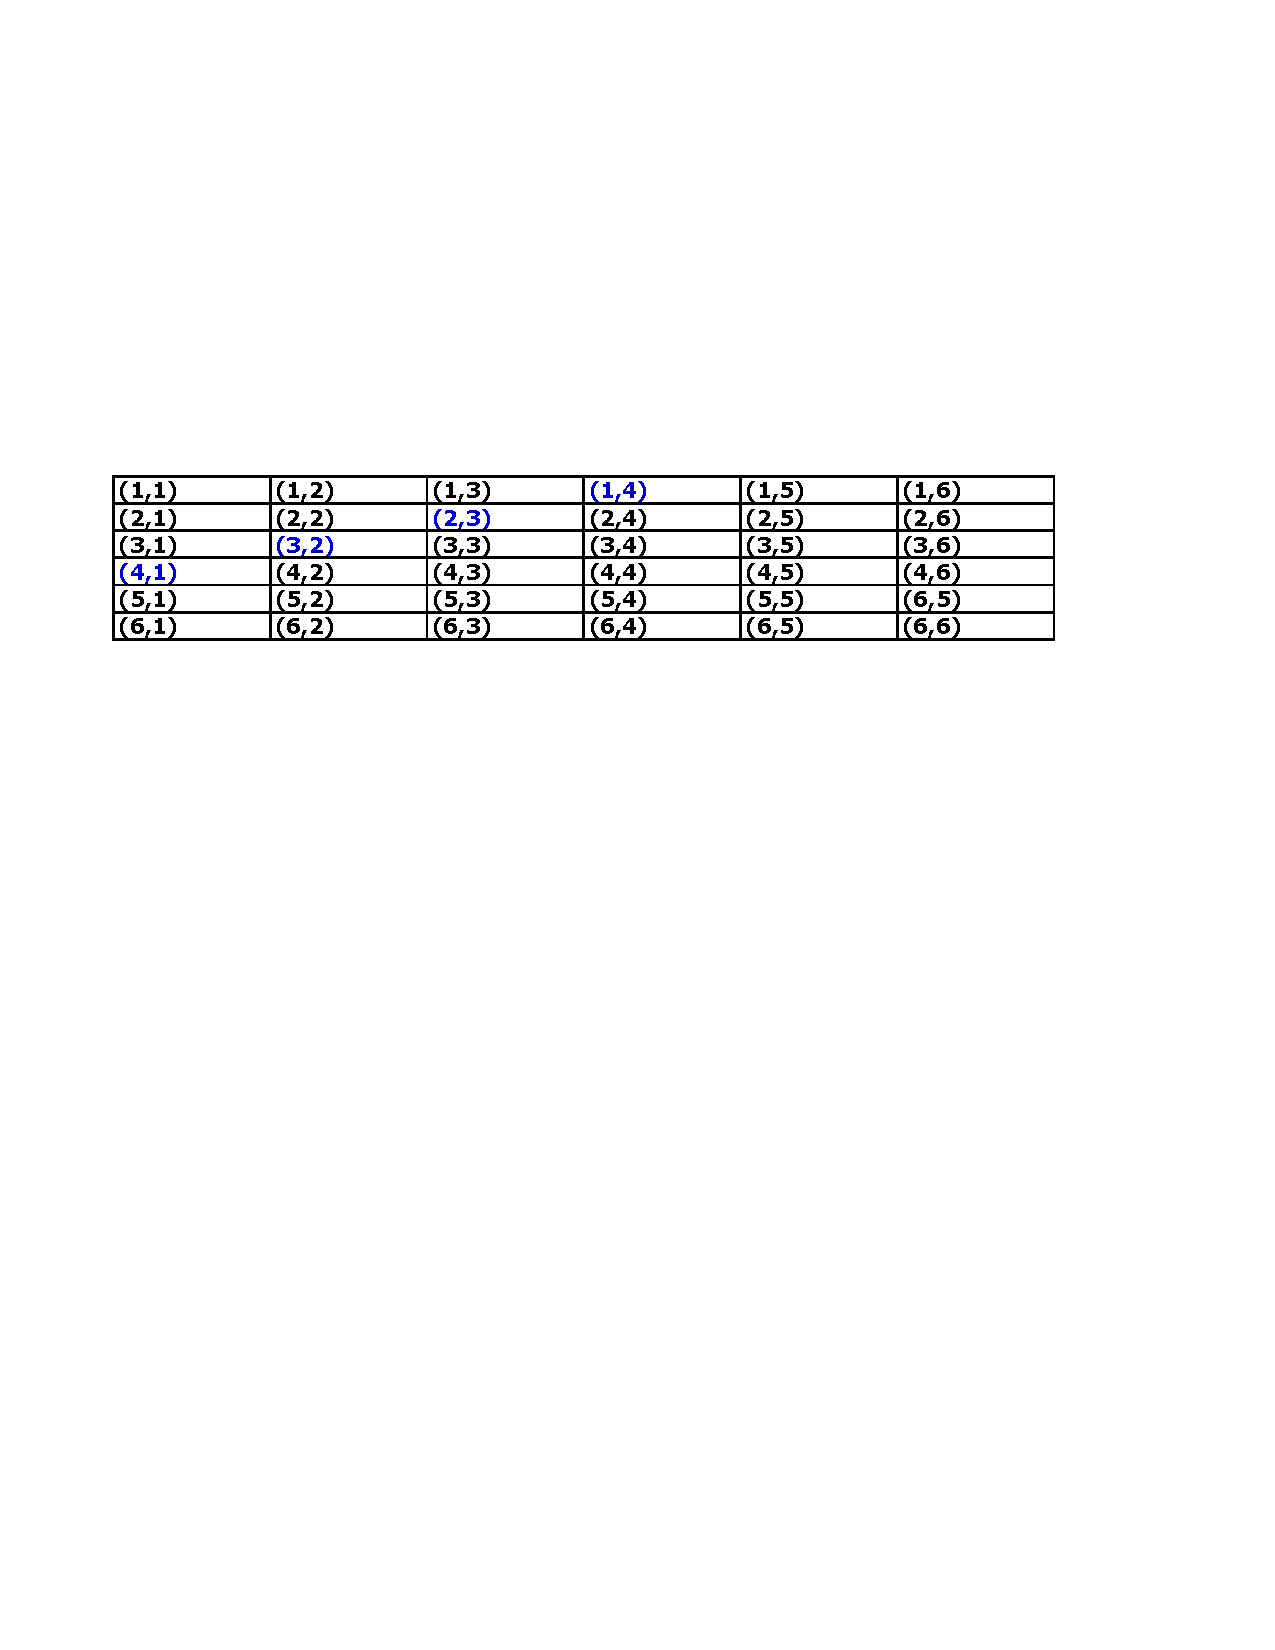
\includegraphics[scale=0.7]{img/c2.pdf}
  \end{figure}
  \end{example}
\end{frame}


\begin{frame}{\secname}

  \begin{example}[cont'd]
  The dice are fair so we can get 36 events with equal probability ${1}\big \slash{36}$. Namely:
  $$
  Pr(i,j) = \frac{1}{36}, \quad \text{for} \quad i,j=1,..,6
  $$
  Thus, we can make use of the highlighted probabilities
  \bea
  P(5) &=& Pr\left\{ (1,4) \cup (2,3) \cup (3,2) \cup  (4,1) \right\} \nn \\
  &=& Pr\left\{ (1,4)  \right\} +  Pr\left\{ (2,3)  \right\} +  Pr\left\{(3,2)  \right\} + Pr\left\{  (4,1) \right\} \nn \\
  &=& {1}\big \slash{36} + {1}\big \slash{36} + {1}\big \slash{36} + {1}\big \slash{36} \nn \\
  &=& {4}\big \slash{36} \nn \\
  &=& 1 \big \slash{9}. \nn
  \eea
  \end{example}
\end{frame}

\begin{frame}{\secname}
  \begin{example}[cont'd]
  Now, suppose that we throw the die first and we get 2.\\
  \vspace{0.2cm}
  \textbf{What is the probability of getting 5 given that we have observed 2 in the first throw?}
  \begin{figure}[h!]
  \centering
  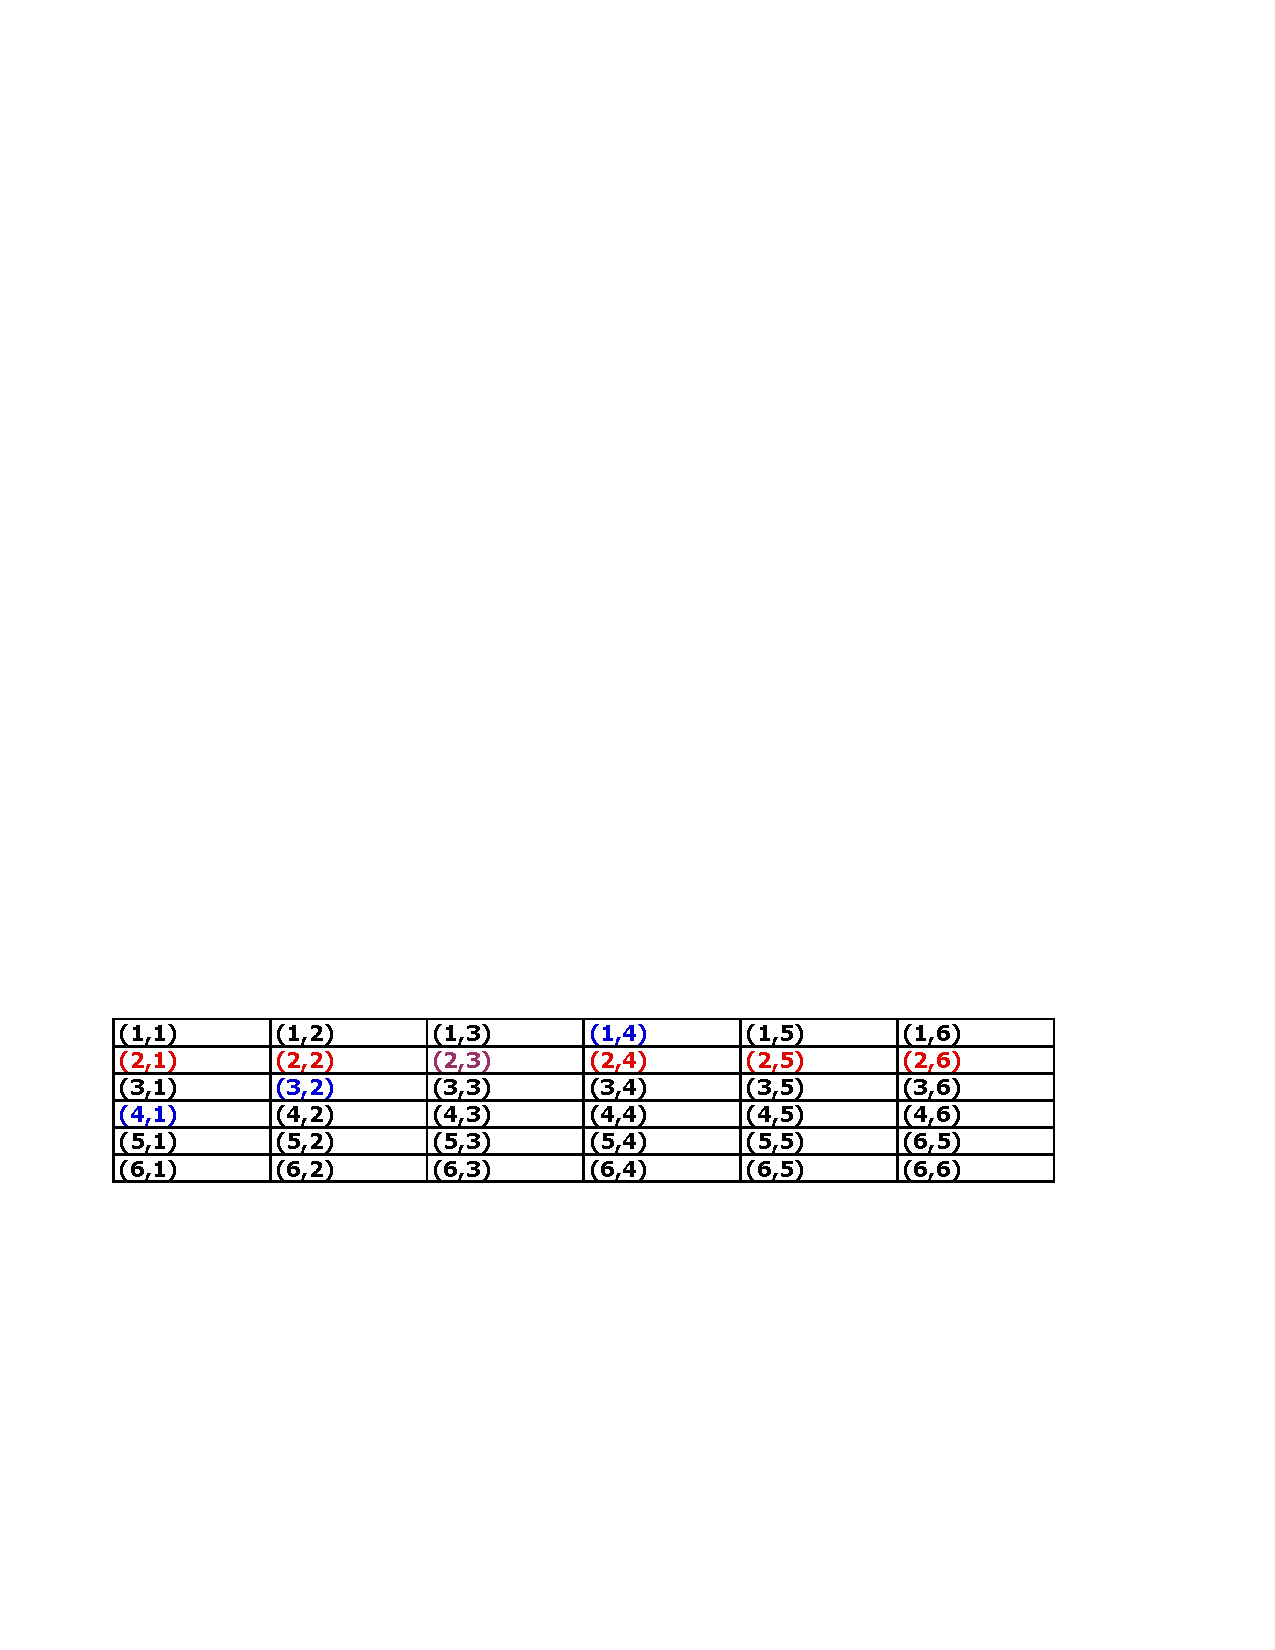
\includegraphics[scale=0.7]{img/c4.pdf}
  \end{figure}
  \begin{footnotesize}
  $\text{Pr}\{\text{getting 5 given 2 in the first throw}\}= \text{Pr}\{\text{getting 3 in the second throw}\}=1/6$
  \end{footnotesize}
  \end{example}
\end{frame}

\begin{frame}{\secname}
  \begin{remark}
  \begin{itemize}
  \item Information changes the probability
  \item By knowing that we got 2 in the first throw, we have changed the sample space:
  \begin{figure}[h!]
  \centering
  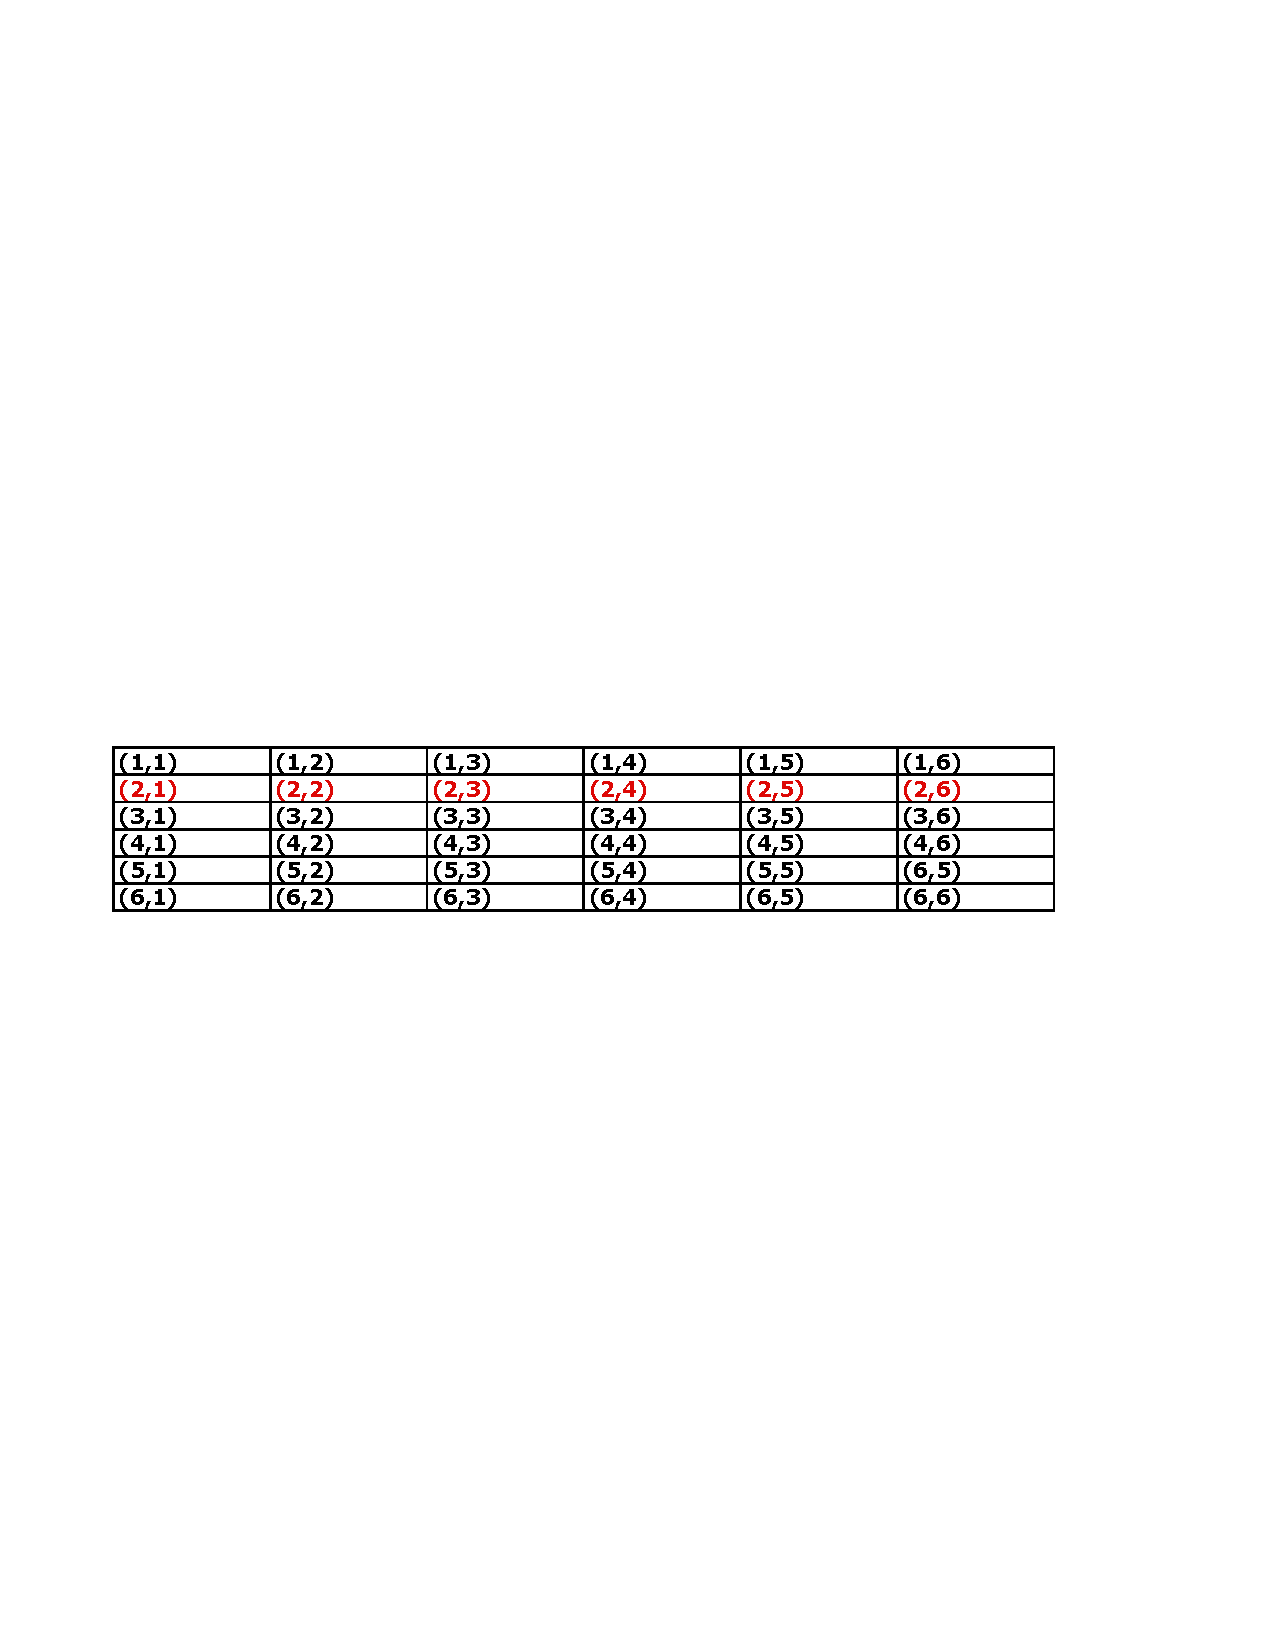
\includegraphics[scale=0.65]{img/c3.pdf}
  \end{figure}
  \item Probability can change drastically --- e.g., suppose that in our example we have 6 in the first throw $\Rightarrow$ the probability of
  observing 5 in two draws ... is zero !!!
  \end{itemize}
  \end{remark}
\end{frame}

\begin{frame}{\secname}

  \begin{definition}
  Let $A$ and $B$ be two events. The conditional probability of event $A$
  given event $B$, denoted by $P\left(A\vert B\right)$, is defined by:
  $$
  P\left(A\vert B\right) = \frac{P(A \cap B)}{P(B)}, \quad \text{if} \quad P(B) >0,
  $$
  and it is left undefined if $P(B)=0$.
  \end{definition}
\end{frame}

\begin{frame}{\secname}

  \begin{example}[A check]
  Let us define the set $B$ as:

  \begin{figure}[h!]
  \centering
  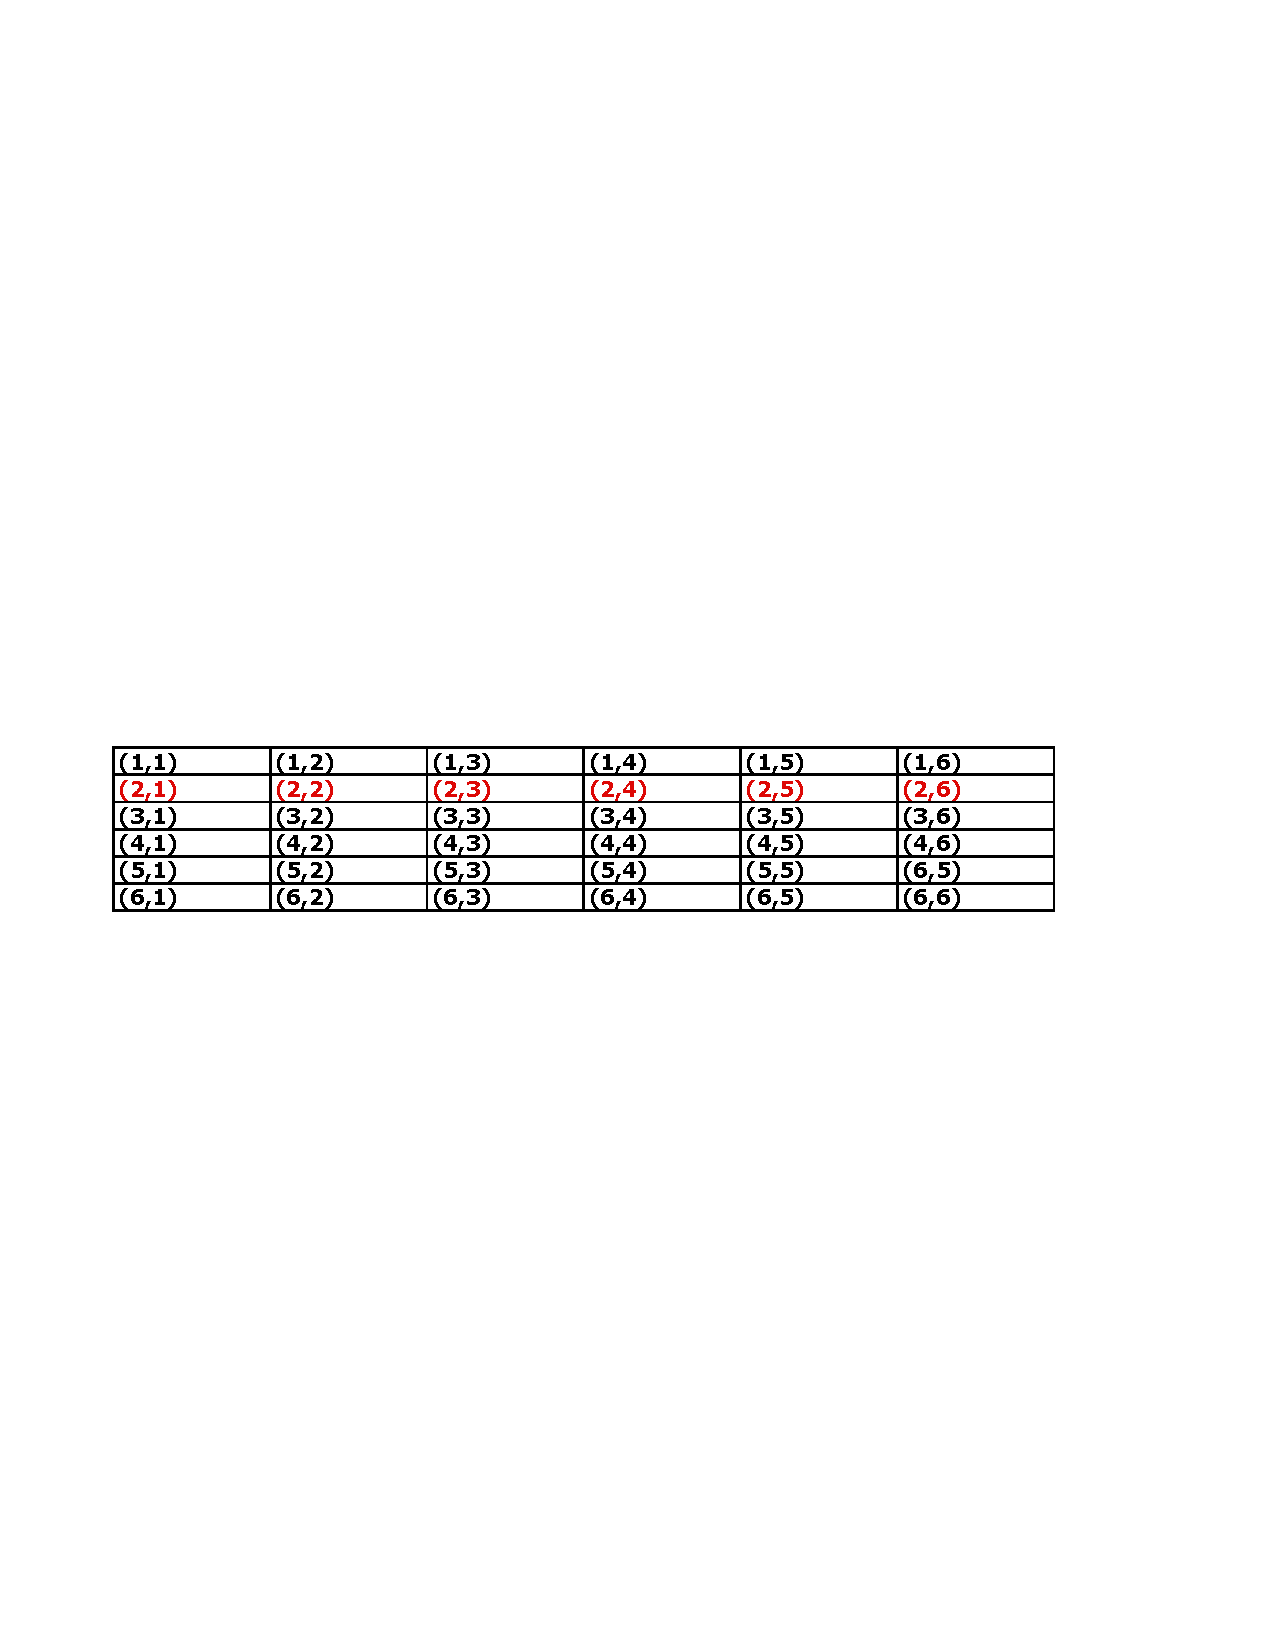
\includegraphics[scale=0.7]{img/c3.pdf}
  \end{figure}
  So we have
  \footnotesize{
  \bea
  P(B) &=& Pr\left\{ (2,1) \cup (2,2) \cup (2,3) \cup (2,4) \cup (2,5) \cup (2,6)     \right\} \nn \\
   &=&  Pr(2,1) + Pr(2,2) + Pr(2,3) + Pr(2,4) + Pr(2,5) + Pr(2,6) \nn \\
   &=& 6/36 =1/6 \nn
  \eea}

  \end{example}
\end{frame}


\begin{frame}{\secname}

  \begin{example} [A check]
  and consider $A \cap B$

  \begin{figure}[h!]
  \centering
  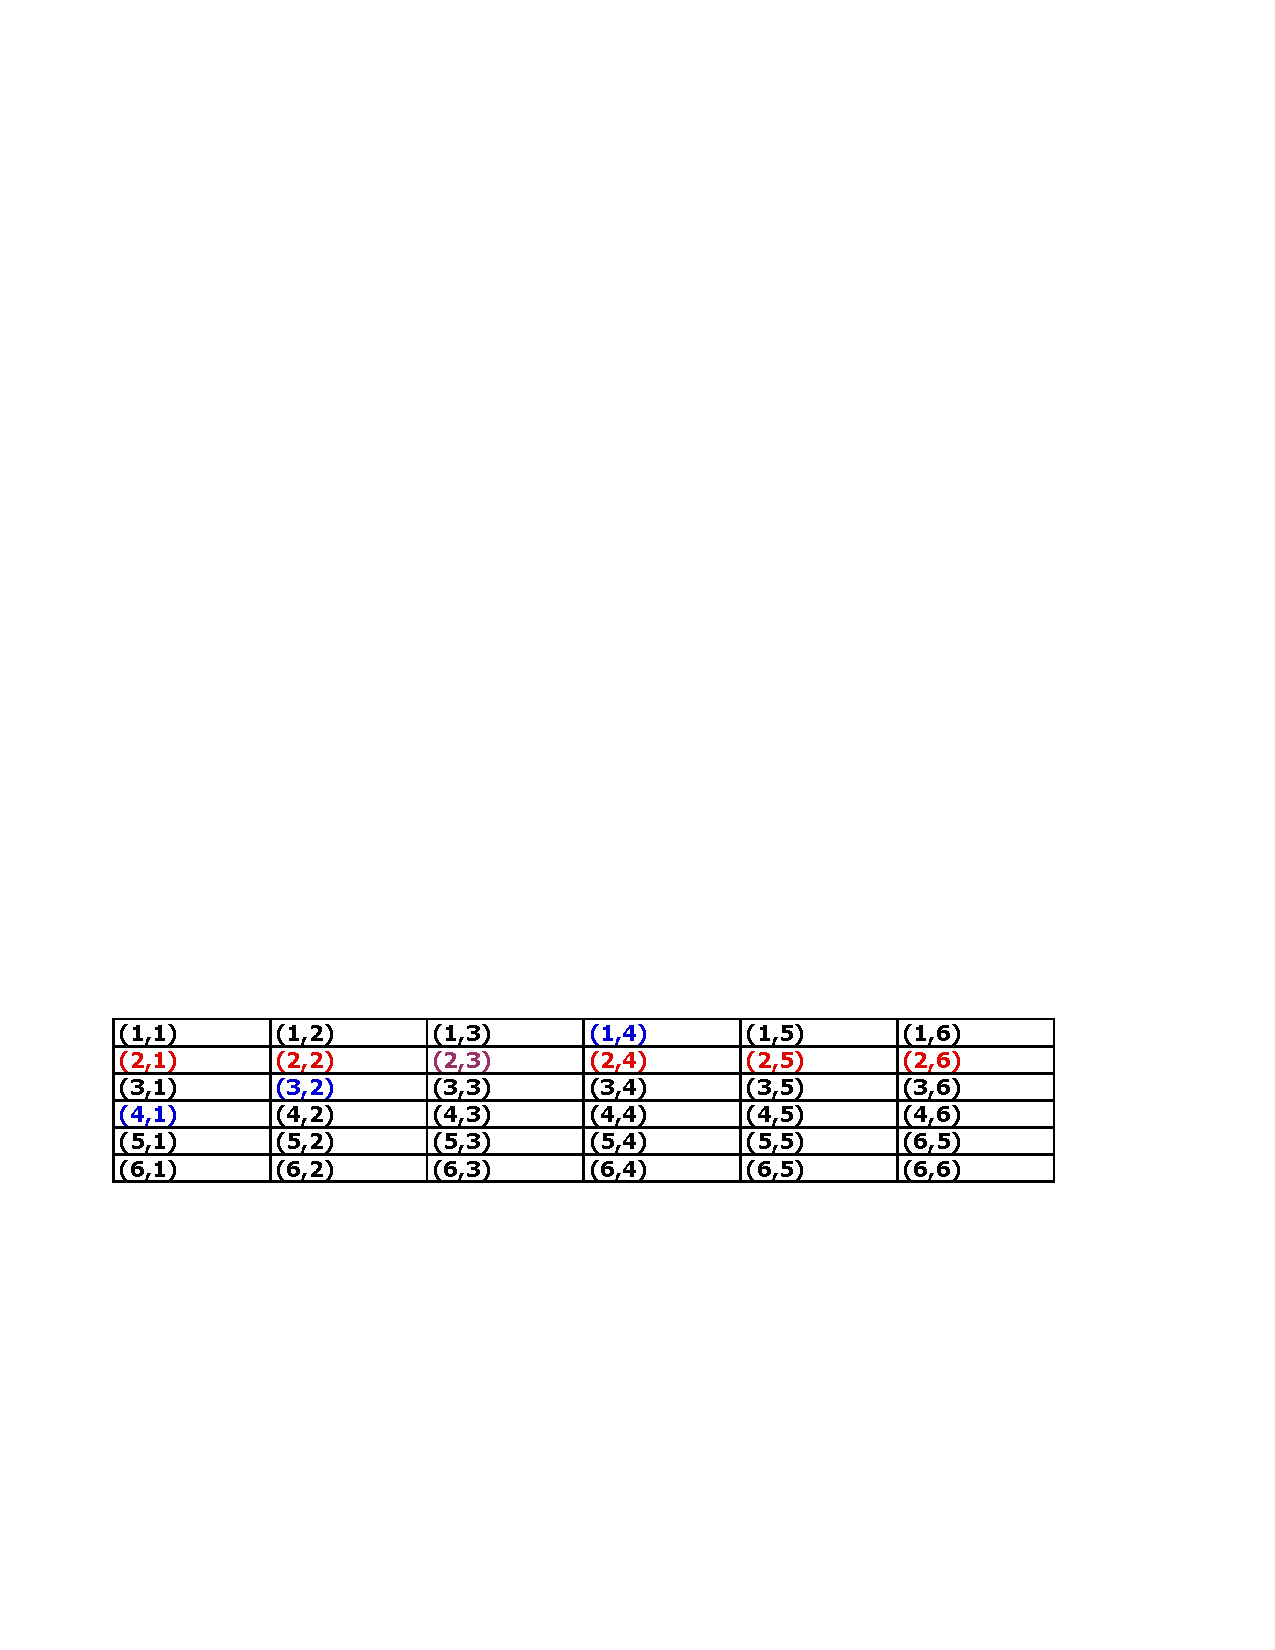
\includegraphics[scale=0.7]{img/c4.pdf}
  \end{figure}
  So we have  $P(A \cap B) = Pr (2,3) = 1/36$ so,
  $$
  P(A\vert B) = \frac{P(A \cap B)}{P(B)}  =  \frac{1/36}{1/6} = \frac{1}{6}. \nn
  $$
  \end{example}
\end{frame}

%%%%%%%%%%%%%%%%%%%%%%%%%%%%%%%%%%%%%%%%%%%%%%%%%%%%%%%%%%%%%%%%%%%%%%%%%%%%%%%%
\section{Independence}
%%%%%%%%%%%%%%%%%%%%%%%%%%%%%%%%%%%%%%%%%%%%%%%%%%%%%%%%%%%%%%%%%%%%%%%%%%%%%%%%

\begin{frame}{\secname}
  \begin{definition}
  Two events $A$ and $B$ are independent if the occurrence of one event has no effect on the probability of occurrence of the other event. Thus,
  $$
  P(A\vert B) = P(A)
  $$
  or equivalently
  $$
  P(B\vert A) = P(B)
  $$
  \end{definition}
  Clearly, if $P(A\vert B) \neq P(A)$, then $A$ and $B$ are \textit{dependent}.
\end{frame}


\begin{frame}{\secname}
  \framesubtitle{A second characterisation}
  Two events $A$ and $B$ are independent if
  $$
  P(A \vert B) = {P(A)},
  $$
  now by definition of conditional probability we know that
  $$
  P(A \vert B) = \frac{P(A \cap B)}{P(B)},
  $$
  so we have
  $$
  P(A) = \frac{P(A \cap B)}{P(B)},
  $$
  and rearranging the terms, we find that two events are independent iif
  $$
  P(A\cap B) = P(A) P(B).
  $$
\end{frame}

\begin{frame}{\secname}
  \begin{example}
  \begin{figure}[h!]
  \centering
  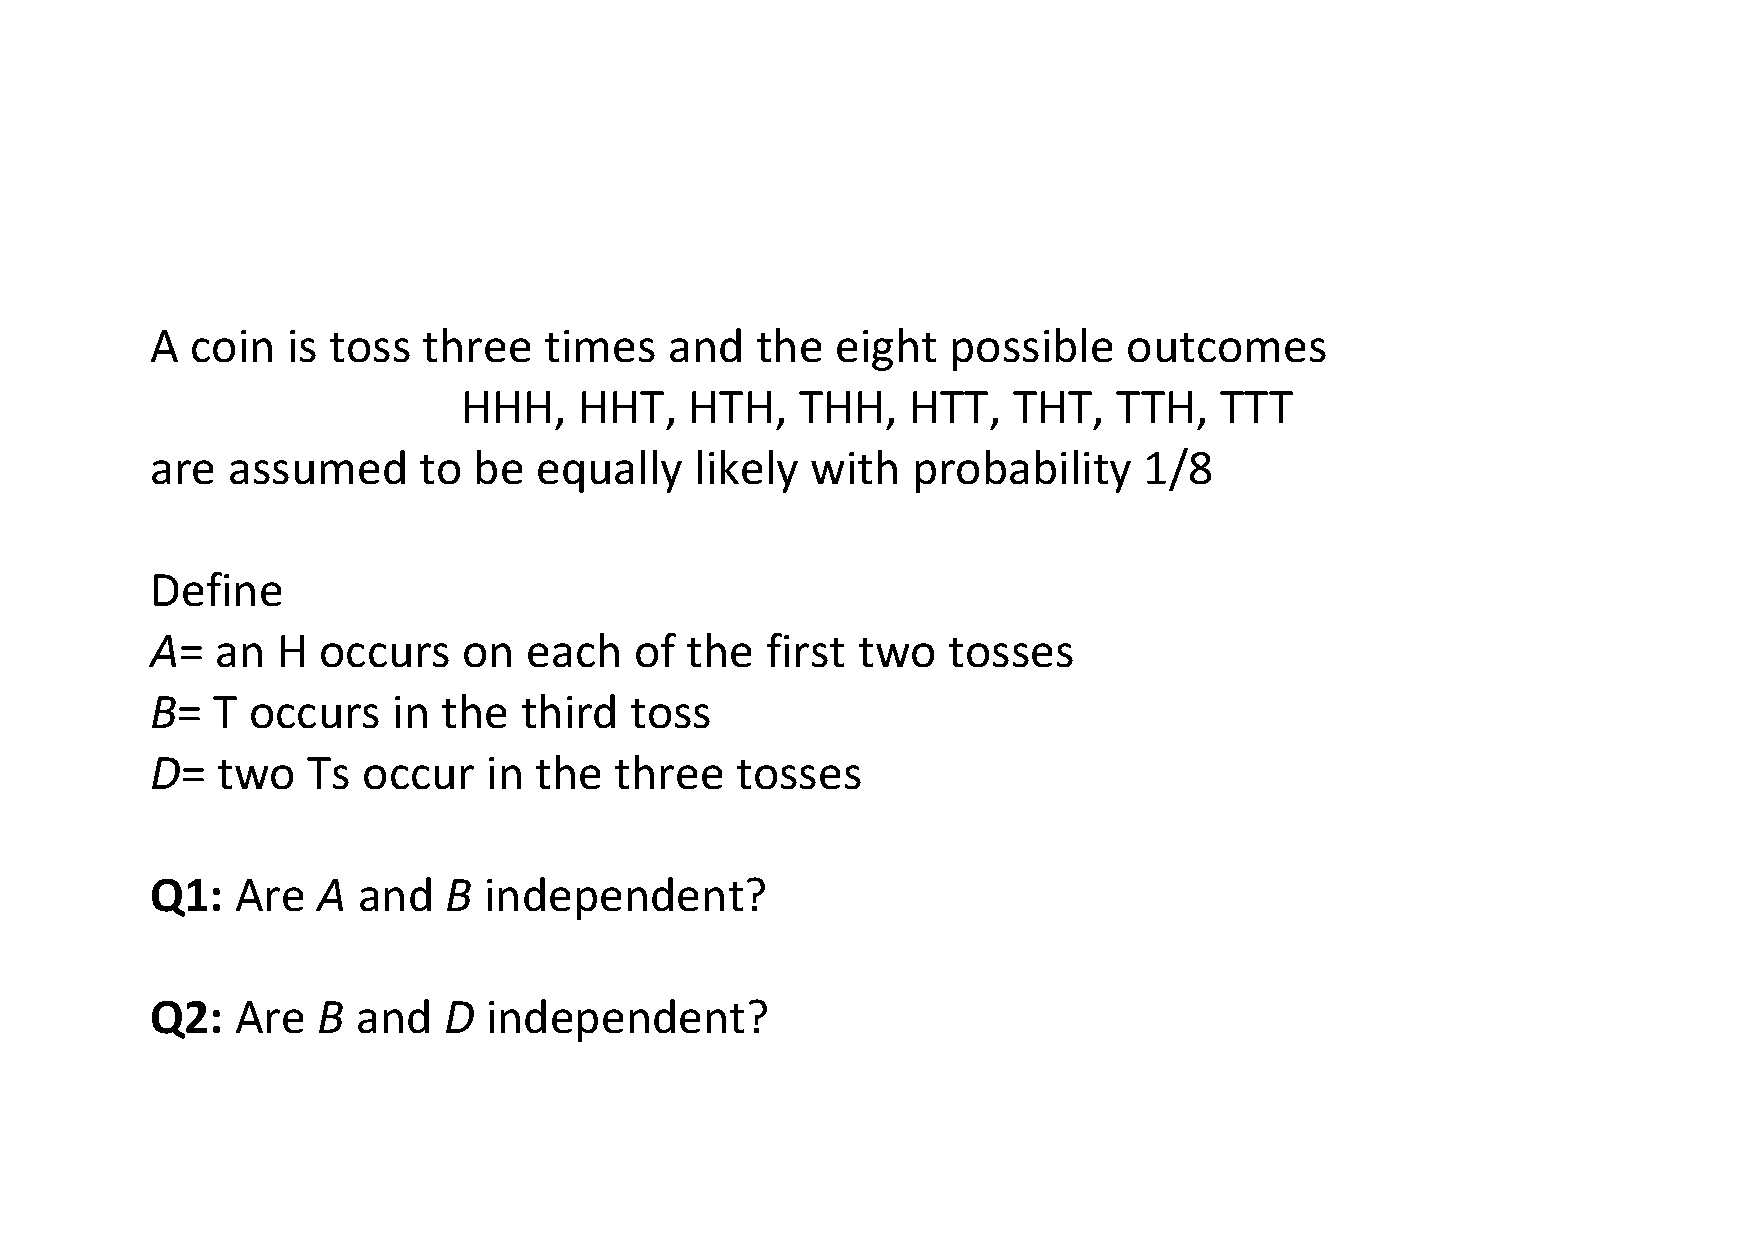
\includegraphics[width=0.9\textwidth,height=0.7\textheight]{img/example7.pdf}
  \end{figure}
  \end{example}
\end{frame}


\begin{frame}{\secname}
  \begin{example}[cont'd]
  \begin{figure}[h!]
  \centering
  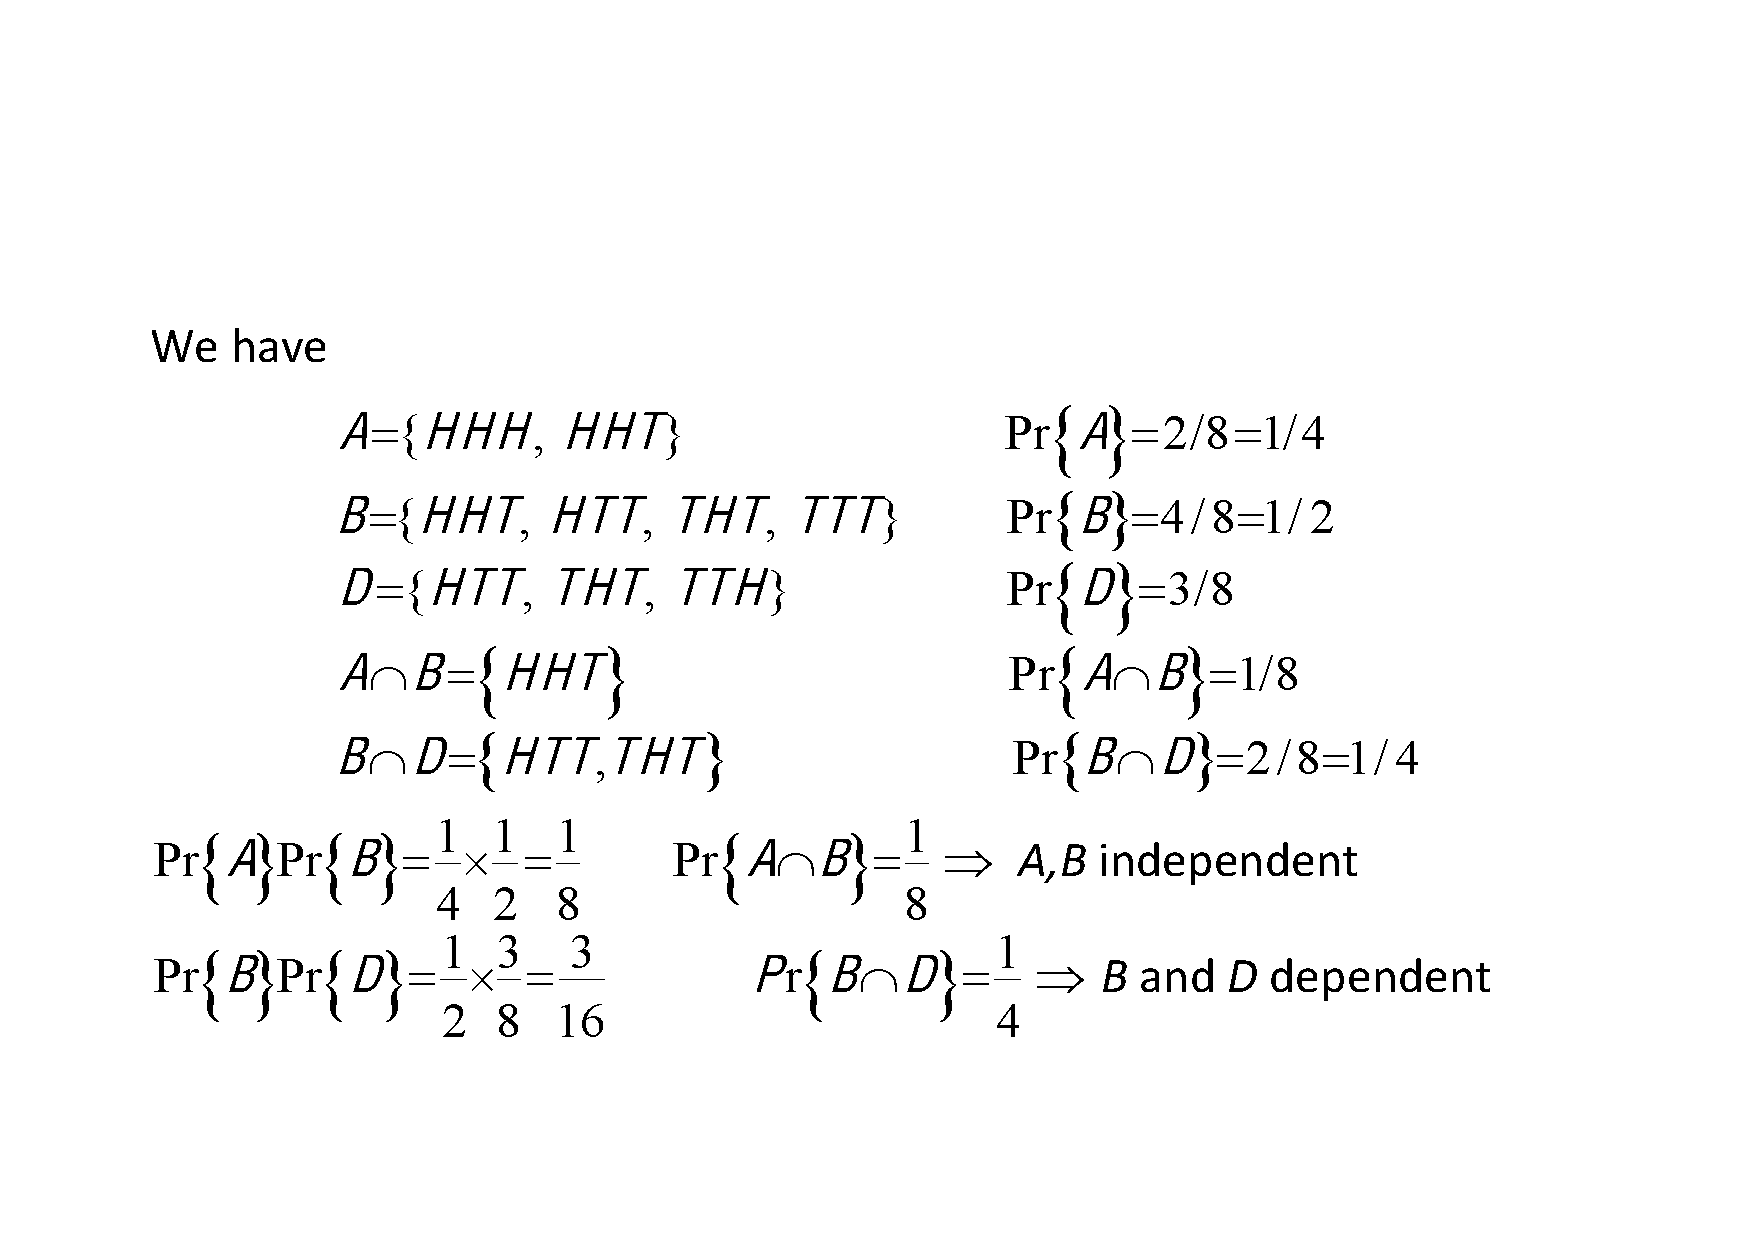
\includegraphics[width=0.9\textwidth,height=0.6\textheight]{img/example8.pdf}
  \end{figure}
  \end{example}
\end{frame}


%%%%%%%%%%%%%%%%%%%%%%%%%%%%%%%%%%%%%%%%%%%%%%%%%%%%%%%%%%%%%%%%%%%%%%%%%%%%%%%%
\section{Theorem I: The Theorem of Total Probability}
%%%%%%%%%%%%%%%%%%%%%%%%%%%%%%%%%%%%%%%%%%%%%%%%%%%%%%%%%%%%%%%%%%%%%%%%%%%%%%%%

\begin{frame}{\secname}
  \begin{theorem}[Total Probabilities]
  \label{Th:totprob}
  Let  $B_1,B_2,...,B_k,...,B_n$ be mutually disjoint events, satisfying
  $S=\cup_{i=1}^{n} B_i,$ and $P(B_i)>0$, for every $i=1,2,...,n$ then for every $A$ we have that:
  \begin{equation}
  \label{TP}
  P(A)=\sum_{i=1}^n P(A\vert B_i) P(B_i).
  \end{equation}
  \end{theorem}

  \begin{footnotesize}
  \begin{proof}
  Write $A=A\cap S = A\cap (\cup_{i=1}^{n} B_i) = \cup_{i=1}^{n} (A\cap B_i)$. Since the $\{B_i \cap A \}$ are mutually disjoint, we have
  \begin{equation*}
  P(A)=P\left(  \cup_{i=1}^{n} (A\cap B_i)  \right)=\sum_{i=1}^n P\left( A\cap B_i  \right ) =\sum_{i=1}^n P(A\vert B_i) P(B_i).
  \end{equation*}
  \end{proof}
  \end{footnotesize}
\end{frame}


\begin{frame}{\secname}
  \textbf{Remark}. The theorem remains valid even if $n=\infty$ in Eq. (\ref{TP}). (Double check, and re-do the proof using $n=\infty$.)
  \begin{corollary}
  %For a given probability space $(S,\mathcal{B},P)$, let $B\in \cal{B}$ satisfy $0<P(B)<1$; then for every $A\in \cal{B}$:
  Let $B$ satisfy $0<P(B)<1$; then for every event $A$:

  \begin{equation*}
  P(A)=P(A\vert B)P(B)+P(A\vert B^c) P(B^c)
  \end{equation*}

  \end{corollary}

  \begin{proof}
  Exercise [Hint: $S=B \cup B^c$].
  \end{proof}
\end{frame}


%%%%%%%%%%%%%%%%%%%%%%%%%%%%%%%%%%%%%%%%%%%%%%%%%%%%%%%%%%%%%%%%%%%%%%%%%%%%%%%%
\section{Theorem II: Bayes' Theorem}
%%%%%%%%%%%%%%%%%%%%%%%%%%%%%%%%%%%%%%%%%%%%%%%%%%%%%%%%%%%%%%%%%%%%%%%%%%%%%%%%


\begin{frame}{\secname}
  Theorem I can be applied to derive the well-celebrated Bayes' Theorem.
  \begin{theorem} [Bayes' Theorem]
  \label{Th:Bayes}
  Let $B_1,B_2,...,B_k,...,B_n$ be mutually disjoint events, satisfying
  $$S=\cup_{i=1}^{n} B_i,$$ and $P(B_i)>0,$
  for every $i=1,2,...,n$. Then for every event $A$ for which $P(A)>0$, we have that
  \begin{equation}
  \label{Bayes}
  P(B_k\vert A)=\frac{P(A\vert B_k)P(B_k)}{\sum_{i=1}^n P(A\vert B_i) P(B_i)}.
  \end{equation}
  \end{theorem}
\end{frame}

\begin{frame}{\secname}
  \begin{proof}
  Let us write
  \bea
  P(B_k\vert A)&=&\frac{P(A\cap B_k)}{P(A)} \nn \\
  &=&\frac{P(A\cap B_k)}{\sum_{i=1}^n P(A\vert B_i) P(B_i)}\nn \\
  &=&\frac{P(A\vert B_k)P(B_k)}{\sum_{i=1}^n P(A\vert B_i) P(B_i)} \nn
  \eea
  That concludes the proof.
  \end{proof}
\end{frame}

\begin{frame}{\secname}
  \begin{example}
  Let us consider a special case, where we have only two events $A$ and $B$.
  \begin{figure}[h!]
  \centering
  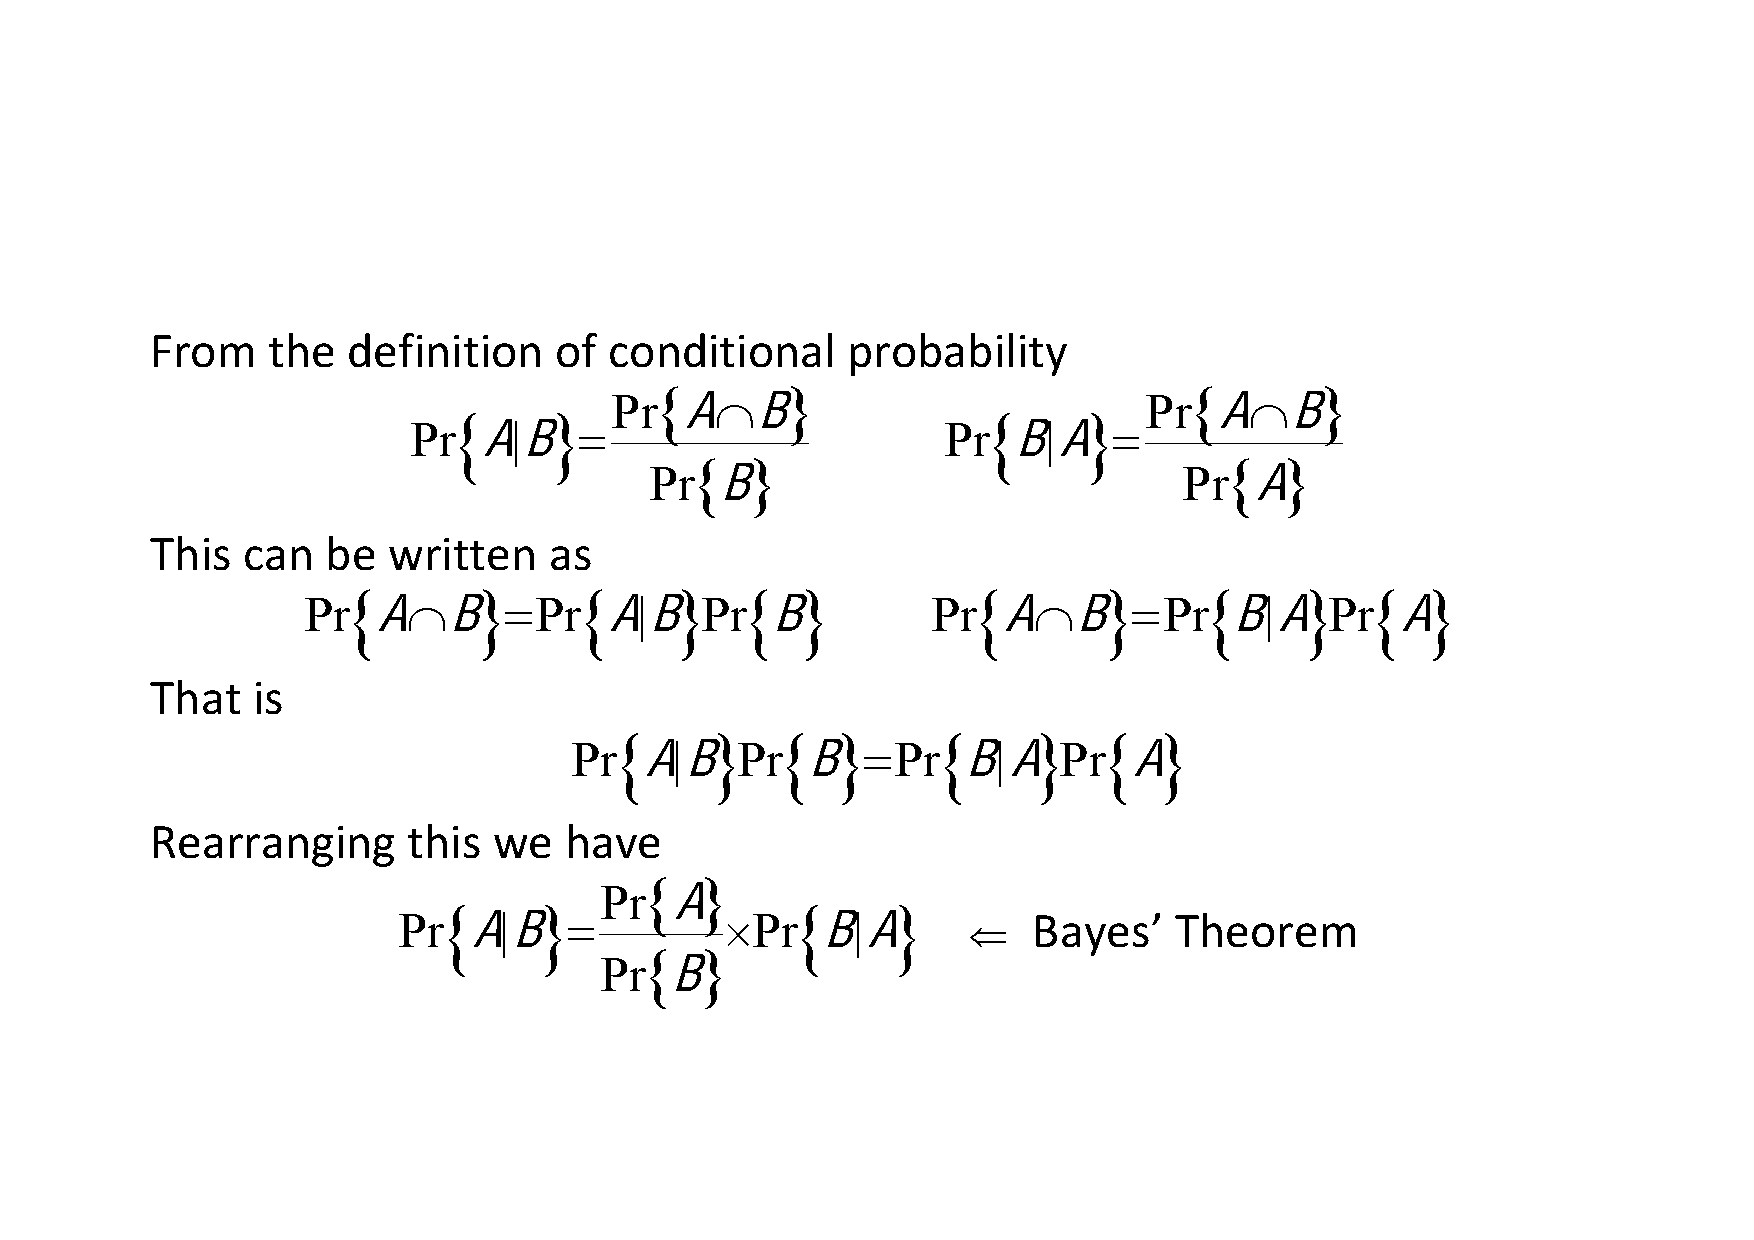
\includegraphics[width=0.9\textwidth,height=0.55\textheight]{img/example10.pdf}
  \end{figure}
  ... so thanks to Bayes' Theorem we can reverse the role of $A\vert B$ and $B \vert A$.
  \end{example}
\end{frame}

%\begin{frame}
%\frametitle{A real-life example}
%\begin{example}
%\begin{figure}[h!]
%\centering
%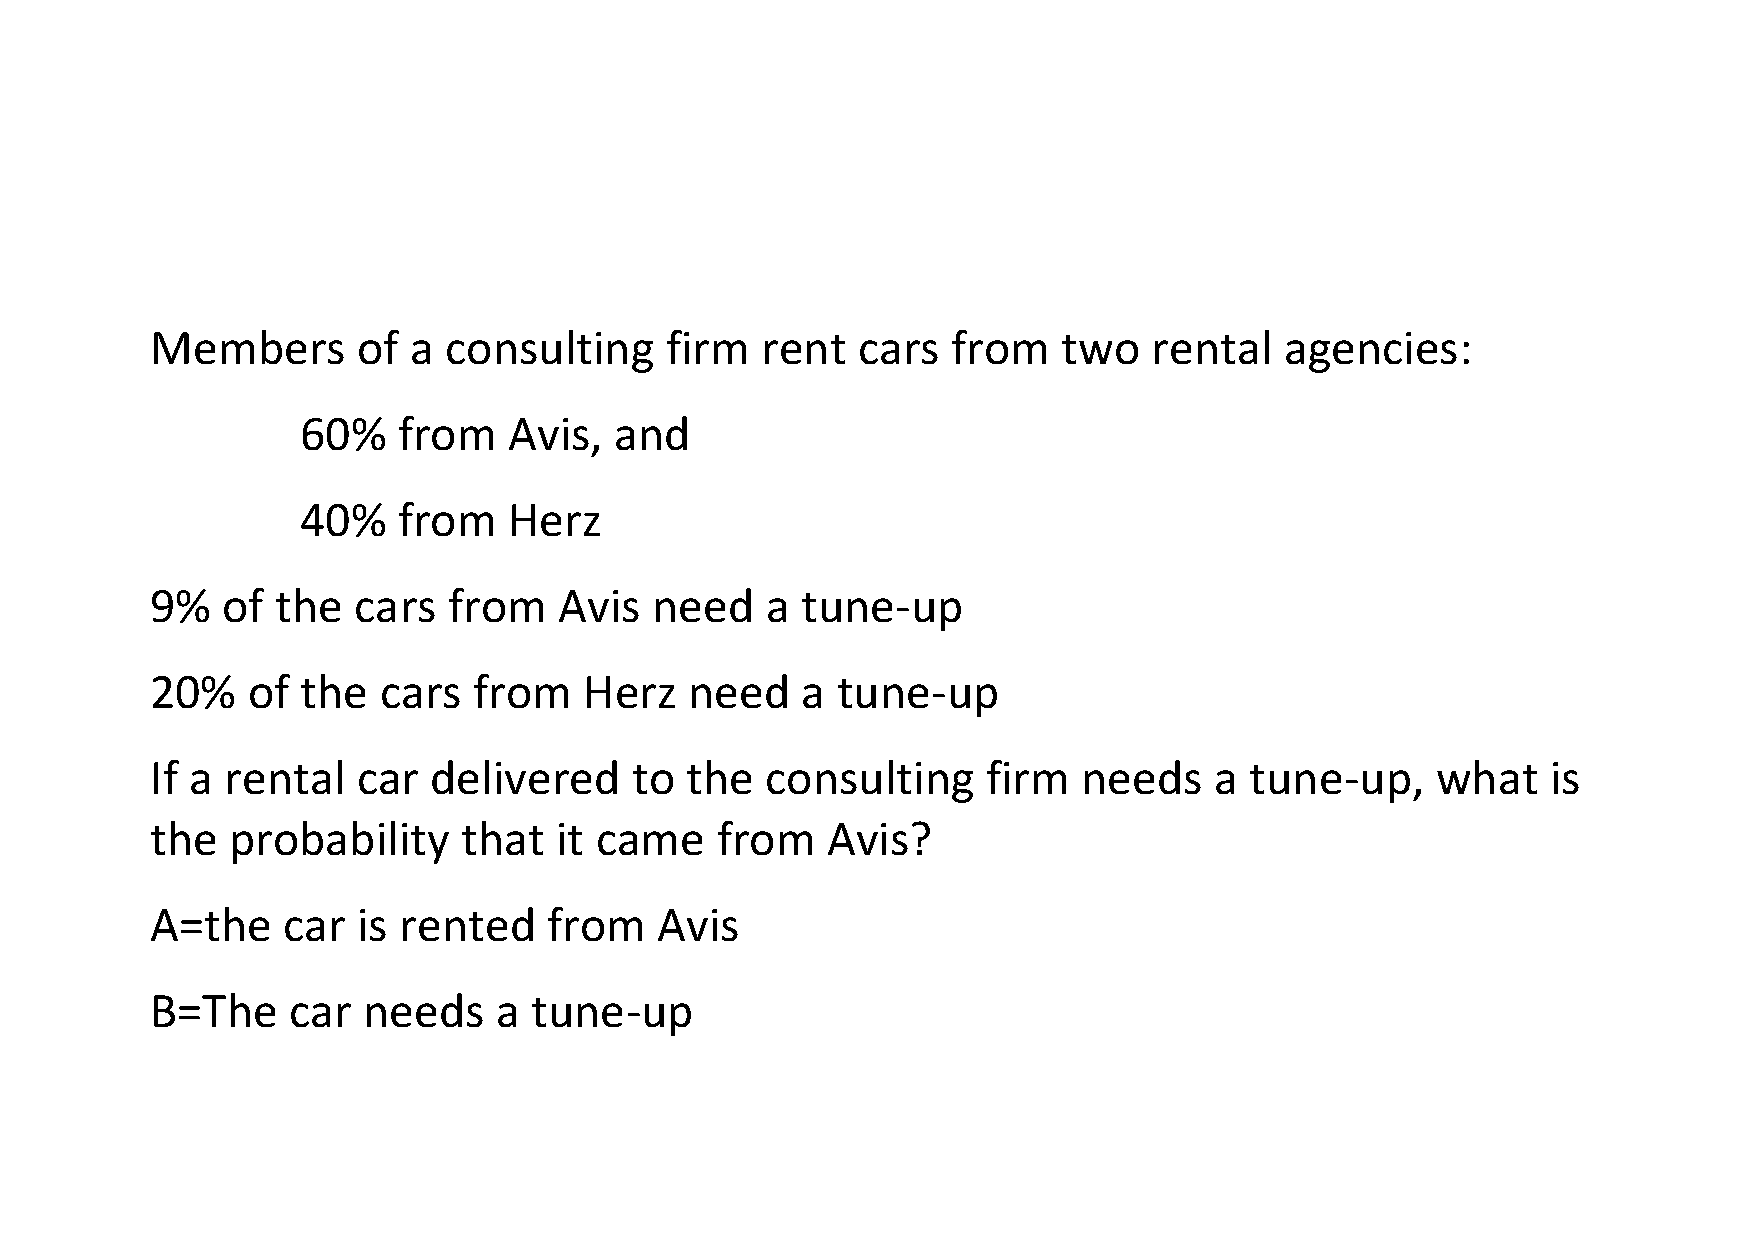
\includegraphics[width=0.9\textwidth,height=0.55\textheight]{img/example9.pdf}
%\end{figure}
%\end{example}
%\begin{aim}
%We know something about $P(B\vert A)$ and we have to say something about $P(A\vert B)$ $\Rightarrow$ Bayes' theorem!!
%\end{aim}
%
%\end{frame}

\begin{frame}{\secname}
\framesubtitle{Application}
  \begin{example}[Guessing in a multiple choice exam]
  \begin{figure}[h!]
  \centering
  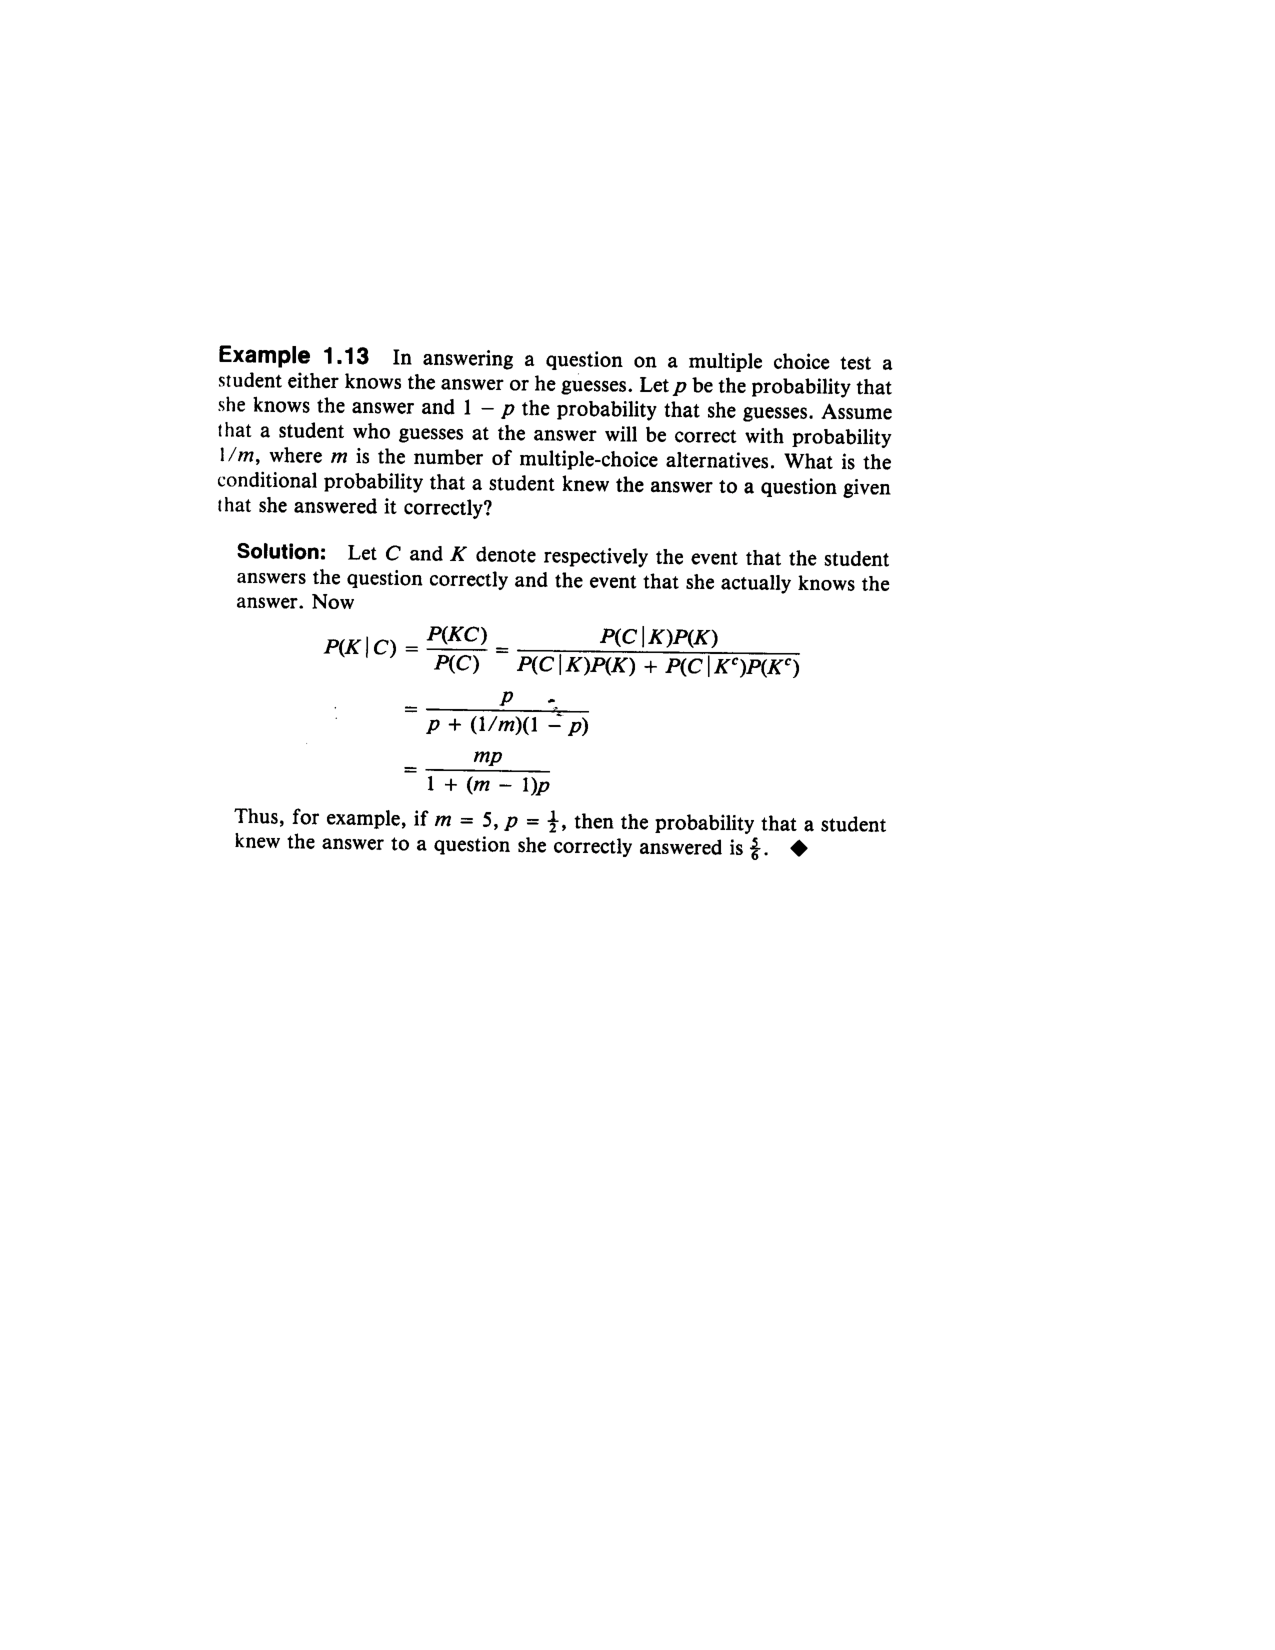
\includegraphics[width=0.7\textwidth,height=0.65\textheight]{img/Ross_Ex.pdf}
  \end{figure}
  \end{example}
\end{frame}

\begin{frame}{\secname}
\framesubtitle{Application}
  \begin{example}
  \begin{footnotesize}
  Members of a consulting firm in Geneva rent cars from two rental agencies:
  \begin{itemize}
  \item 60\% from AVIS
  \item 40\% from Mobility
  \end{itemize}
  Now consider that
  \begin{itemize}
  \item 9\% of the cars from AVIS need a tune-up
  \item 20\% of the cars from Mobility need a tune-up
  \end{itemize}
  If a car delivered to the consulting firm needs a tune-up, what is the probability that the care came
  from AVIS?
  \end{footnotesize}
  \end{example}
  \begin{aim}
  \begin{footnotesize}
  $A:=\{\text{car rented from AVIS}\}$ and $B:=\{\text{car needs a tune-up}\}$. We know $P(B\vert A)$ and we look for $P(A\vert B)$ $\Rightarrow$ Bayes' theorem!!
  \end{footnotesize}
  \end{aim}
\end{frame}

\begin{frame}{\secname}
\framesubtitle{Application}
  \begin{example}[cont'd]
  \begin{figure}[h!]
  \centering
  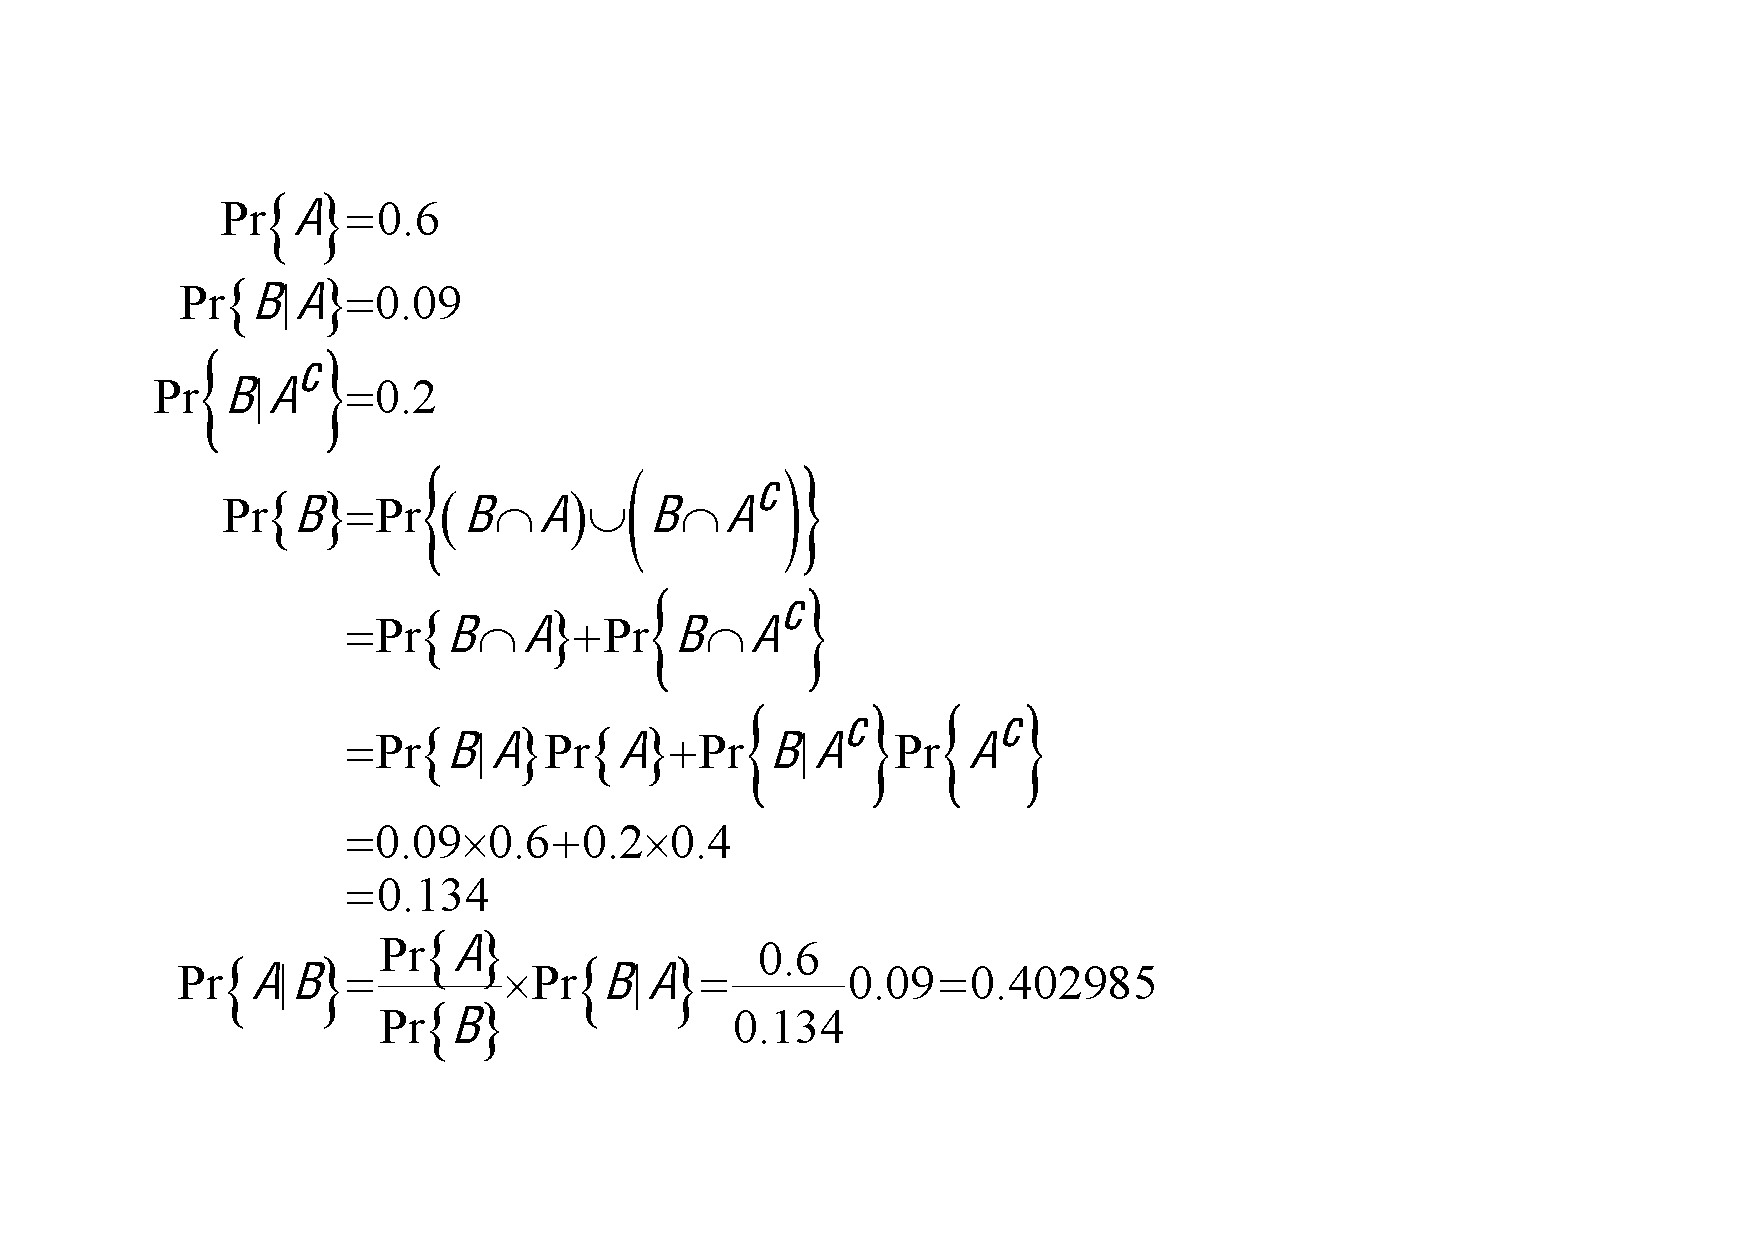
\includegraphics[width=0.9\textwidth,height=0.65\textheight]{img/example9b.pdf}
  \end{figure}
  \end{example}
\end{frame}

%%%%%%%%%%%%%%%%%%%%%%%%%%%%%%%%%%%%%%%%%%%%%%%%%%%%%%%%%%%%%%%%%%%%%%%%%%%%%%%%

\begin{frame}{Wrap-up}

Take-home message

\begin{itemize}
\item The Probability Axioms are important, since they imply \textbf{computation rules}.
\item These rules are key to compute probabilities ``in real life''.
\item Probability of an event can be \textbf{conditional} on the realisation of another event.
\item When an event has the \textbf{same probability} regardless of another it is called independent
\item Theorem I (basic) $$P(A)=P(A \cap B)+P(A\cap B^c) = P(A\vert B)P(B)+P(A\vert B^c) P(B^c)$$
\item Theorem II (basic) If we have $P(A|B)$, we can find $P(B|A)$
$$P(B|A) = \frac{P(A|B)P(B)}{P(A|B)P(B) + P(A|B^c)P(B^c)}$$
\end{itemize}
\end{frame}

\begin{frame}
	\begin{center}

		\LARGE{Thank you for your attention!}

		\pause

		\LARGE{``See you" next week!}
	\end{center}
\end{frame}



\end{document}

